\chapter{Dokumentacja użytkownika aplikacji ExpensePredictor}
W niniejszym rozdziale opisany został interfejs użytkownika oraz funkcjonalność systemu ExpensePredictor. Diagram wszystkich przypadków użycia przedstawiony jest na Rys. \ref{usecases}.
\section{Moduł obsługi konta użytkownika}
Moduł obsługi konta użytkownika swoim zakresem obejmuje pięć przypadków użycia:
\begin{itemize}
	\item zarejestruj,
	\item zaloguj,
	\item wyświetl swoje dane,
	\item edytuj swoje dane,
	\item zmień swoje hasło.
\end{itemize}
\textbf{Rejestracja} (przypadek użycia "zarejestruj") to proces tworzenia nowego konta użytkownika. Jest jedną z dwóch funkcjonalności niewymagających uwierzytelnienia i dostępnych przy pierwszym uruchomieniu aplikacji. Po wybraniu na ekranie startowym (Rys. \ref{ekran_startowy_rejestracja}) przycisku "SIGN UP" otwarta zostaje strona rejestracji (Rys. \ref{rejestracja}). Po poprawnym wypełnieniu pól i naciśnięciu przycisku "SIGN UP" konto zostaje utworzone.
\begin{figure}[!ht]
	\begin{center}
		\begin{subfigure}[b]{0.3\textwidth}
				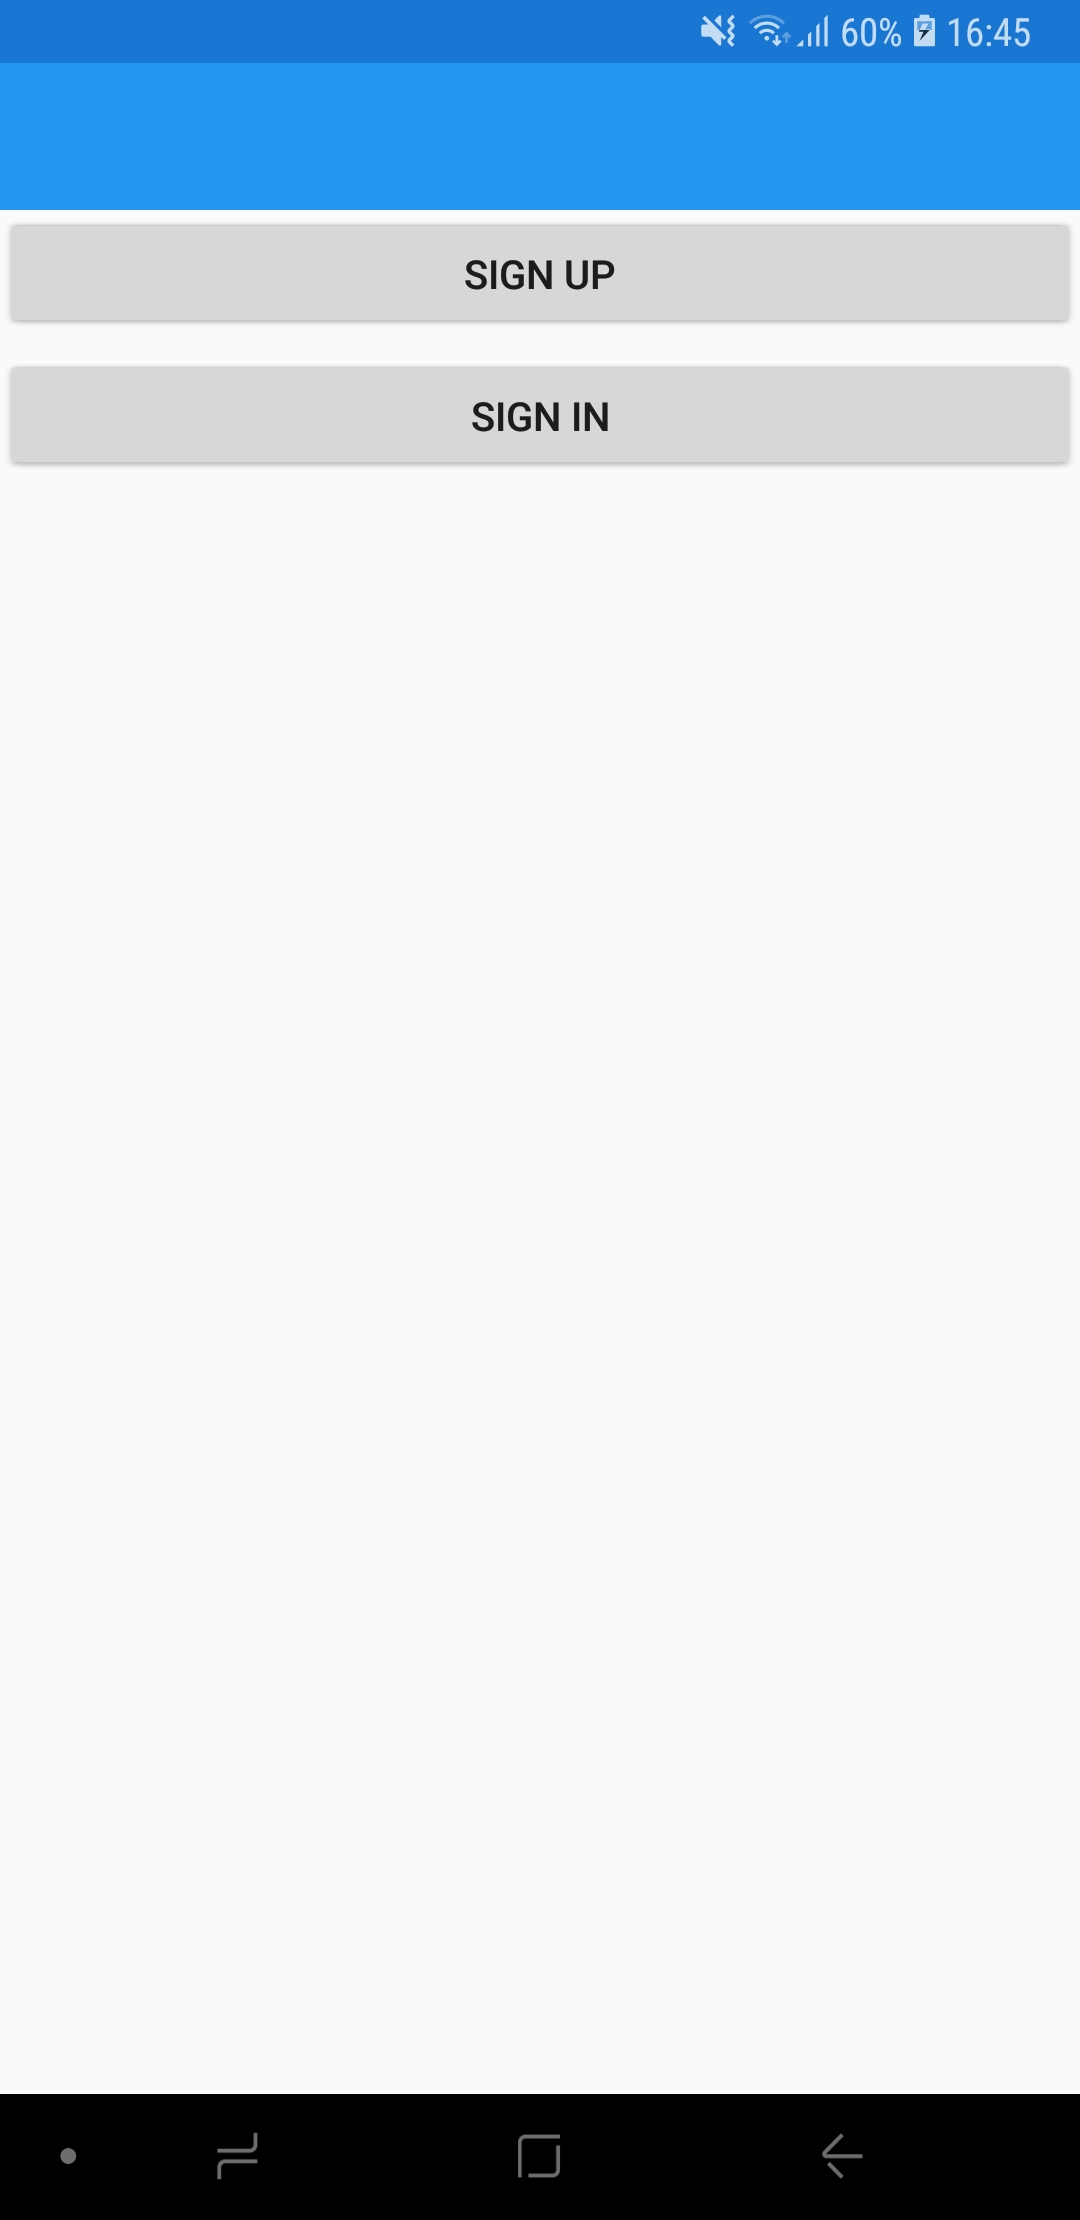
\includegraphics[width=1.75in]{img/mobile/ekran_startowy.jpg}
				\subcaption{Ekran startowy.}
				\label{ekran_startowy_rejestracja}
		\end{subfigure}
		\begin{subfigure}[b]{0.3\textwidth}
				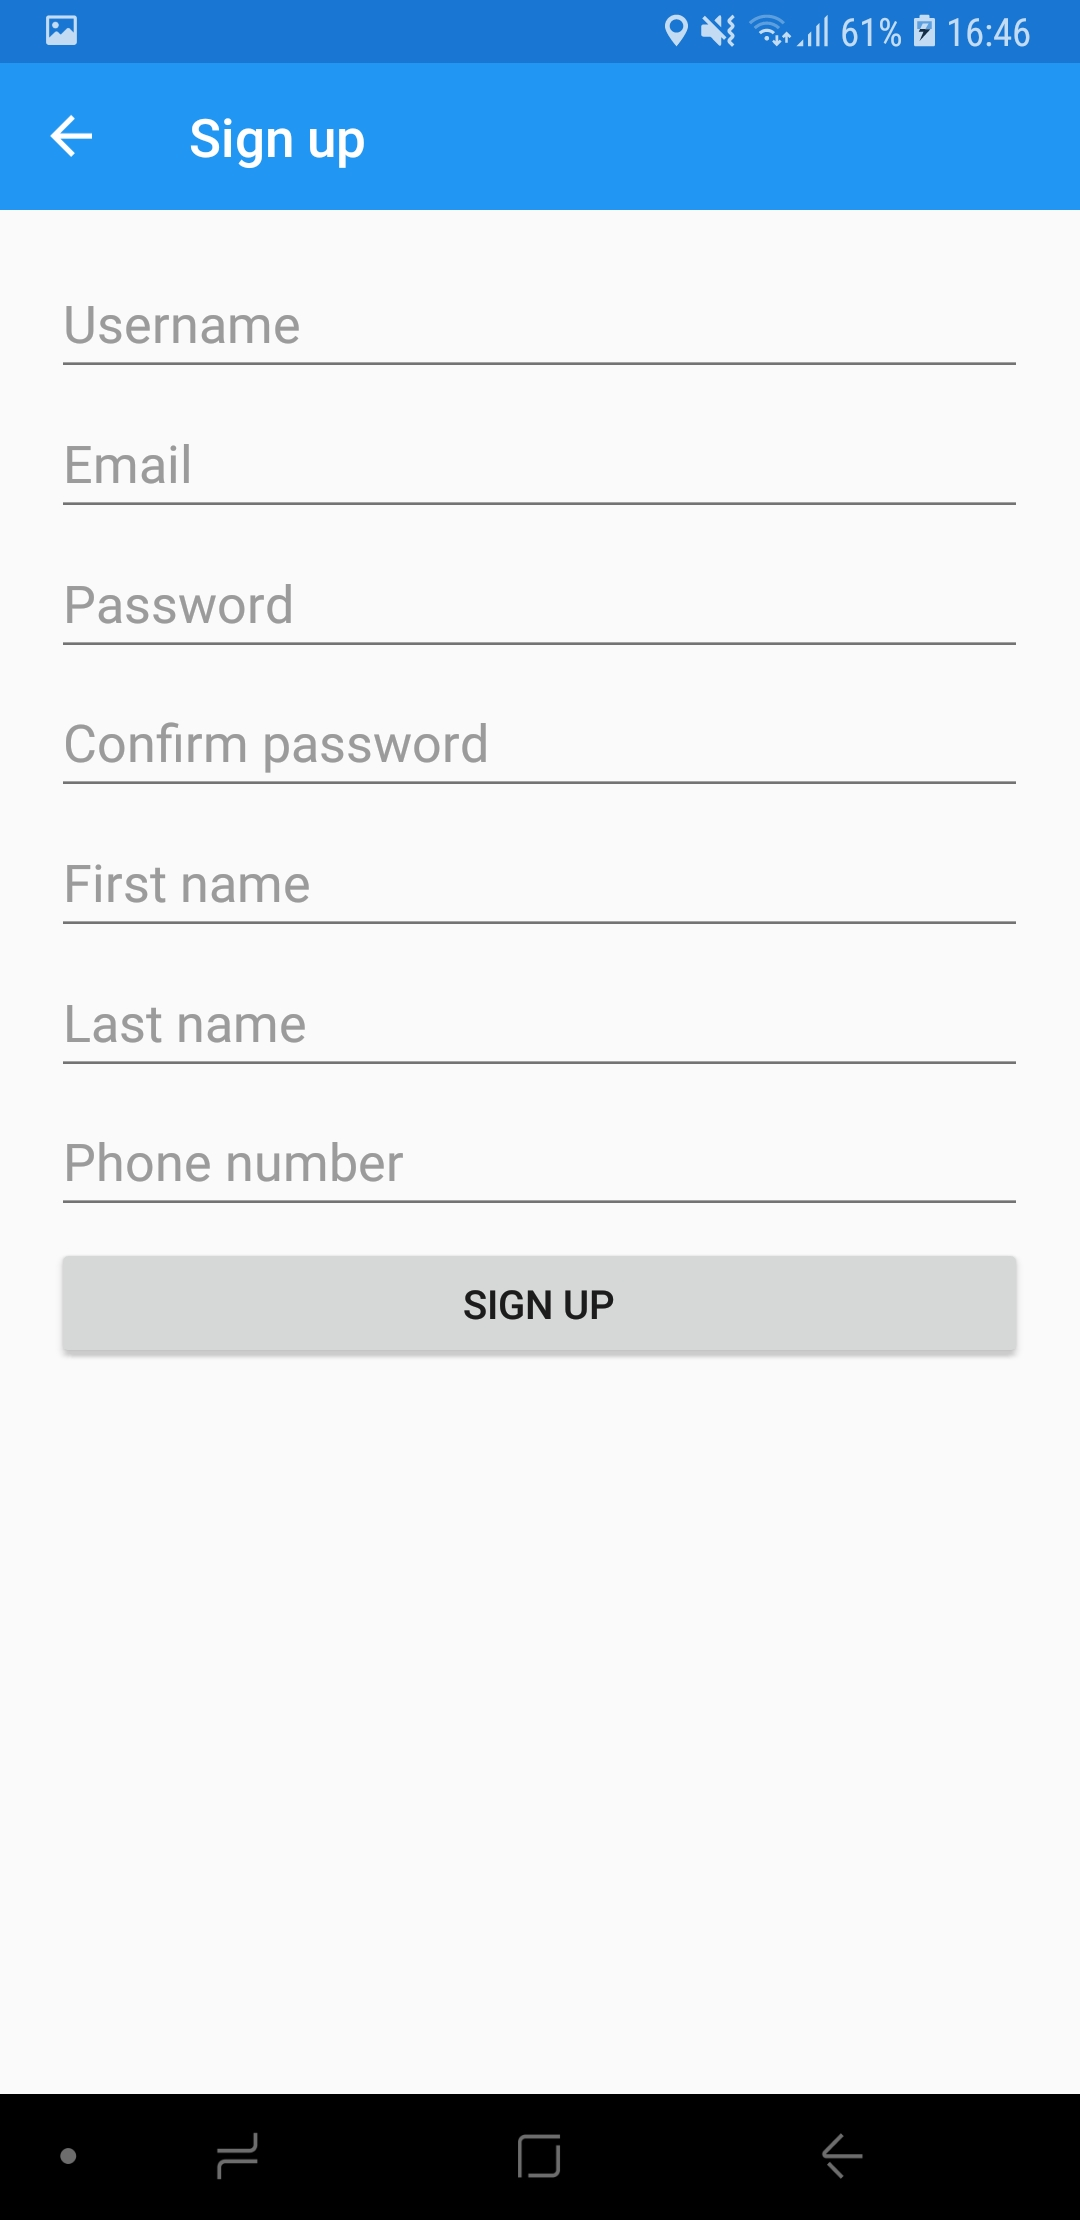
\includegraphics[width=1.75in]{img/mobile/rejestracja.jpg}
				\subcaption{Strona rejestracji.}
				\label{rejestracja}
		\end{subfigure}
	\end{center}
	\caption{Zrzuty ekranu procesu rejestracji.}
\end{figure}

\textbf{Logowanie} (przypadek użycia "zaloguj") jest procesem generacji tokenu uwierzytelniającego. Po wybraniu na ekranie startowym (Rys. \ref{ekran_startowy_logowanie}) przycisku "SIGN IN" wyświetla się strona logowania (Rys. \ref{logowanie}). Po wypełnieniu formularza i wciśnięciu przycisku "SIGN IN", w przypadku błędnego hasła wyświetla się komunikat (Rys. \ref{logowanie_haslo}), w przeciwnym wypadku proces kończy się powodzeniem.
\begin{figure}[!ht]
	\begin{center}
		\begin{subfigure}[b]{0.3\textwidth}
			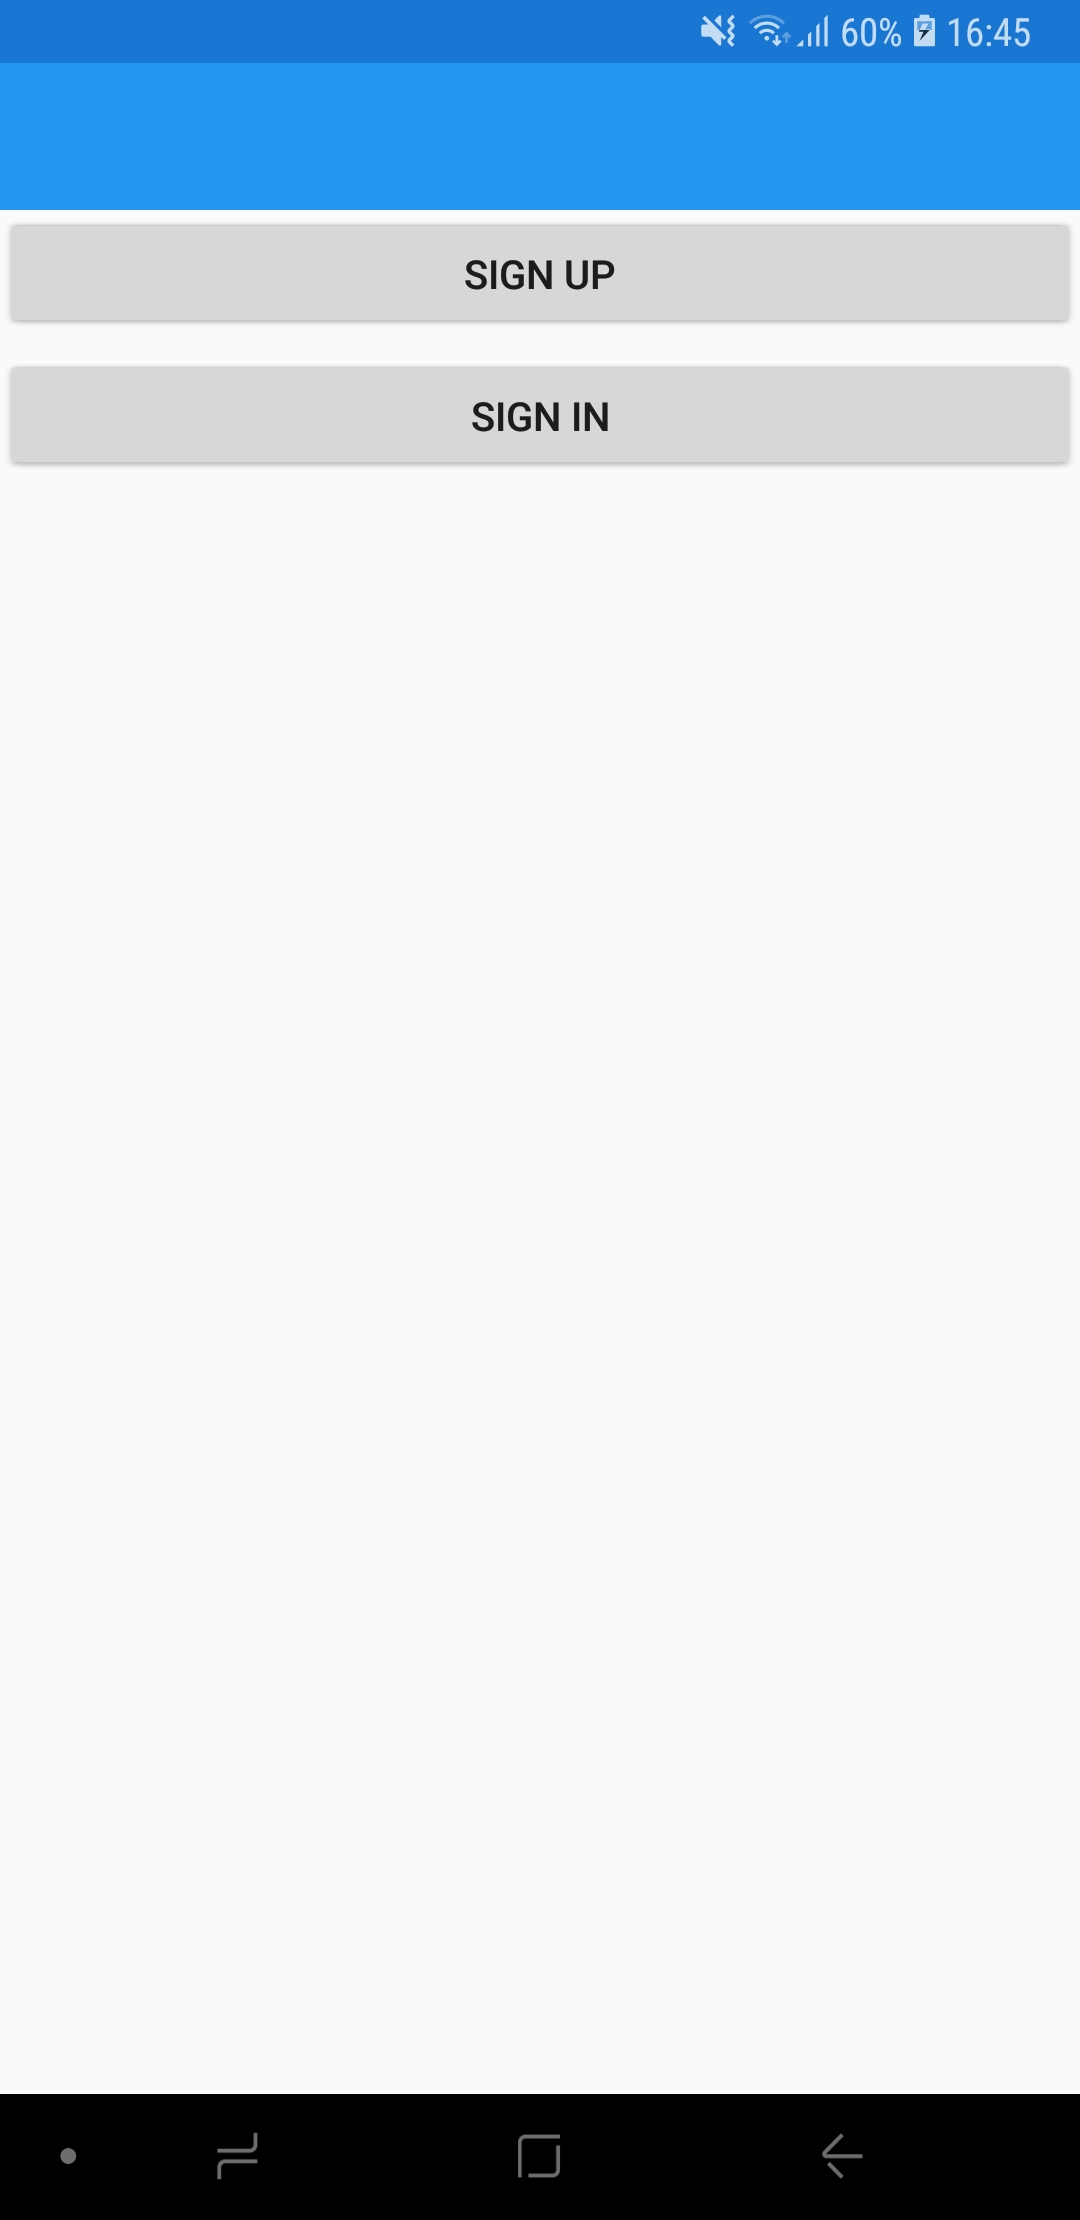
\includegraphics[width=1.75in]{img/mobile/ekran_startowy.jpg}
			\subcaption{Ekran startowy.}
			\label{ekran_startowy_logowanie}
		\end{subfigure}
		\begin{subfigure}[b]{0.3\textwidth}
			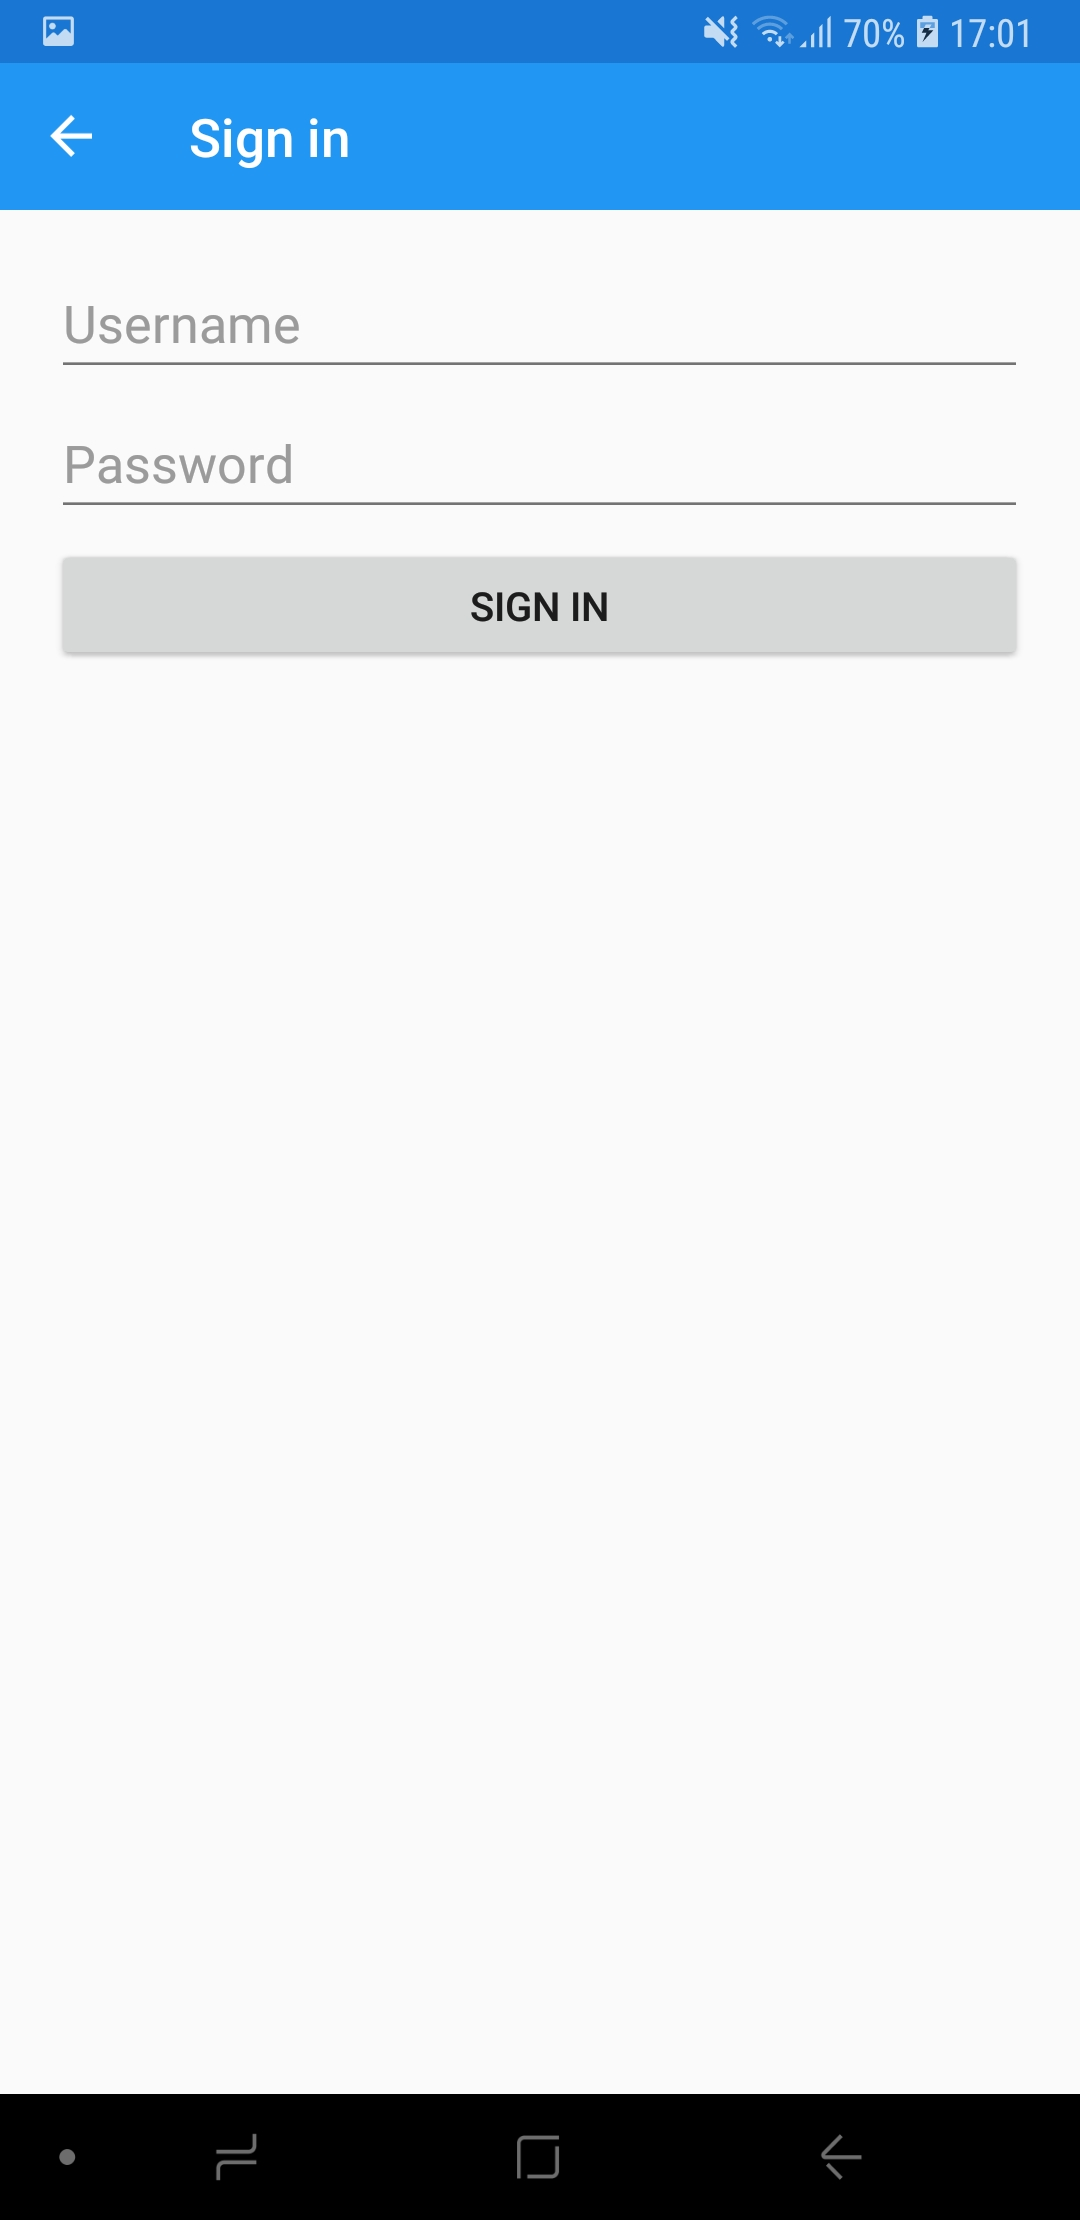
\includegraphics[width=1.75in]{img/mobile/login.jpg}
			\subcaption{Strona logowania.}
			\label{logowanie}
		\end{subfigure}
		\begin{subfigure}[b]{0.3\textwidth}
			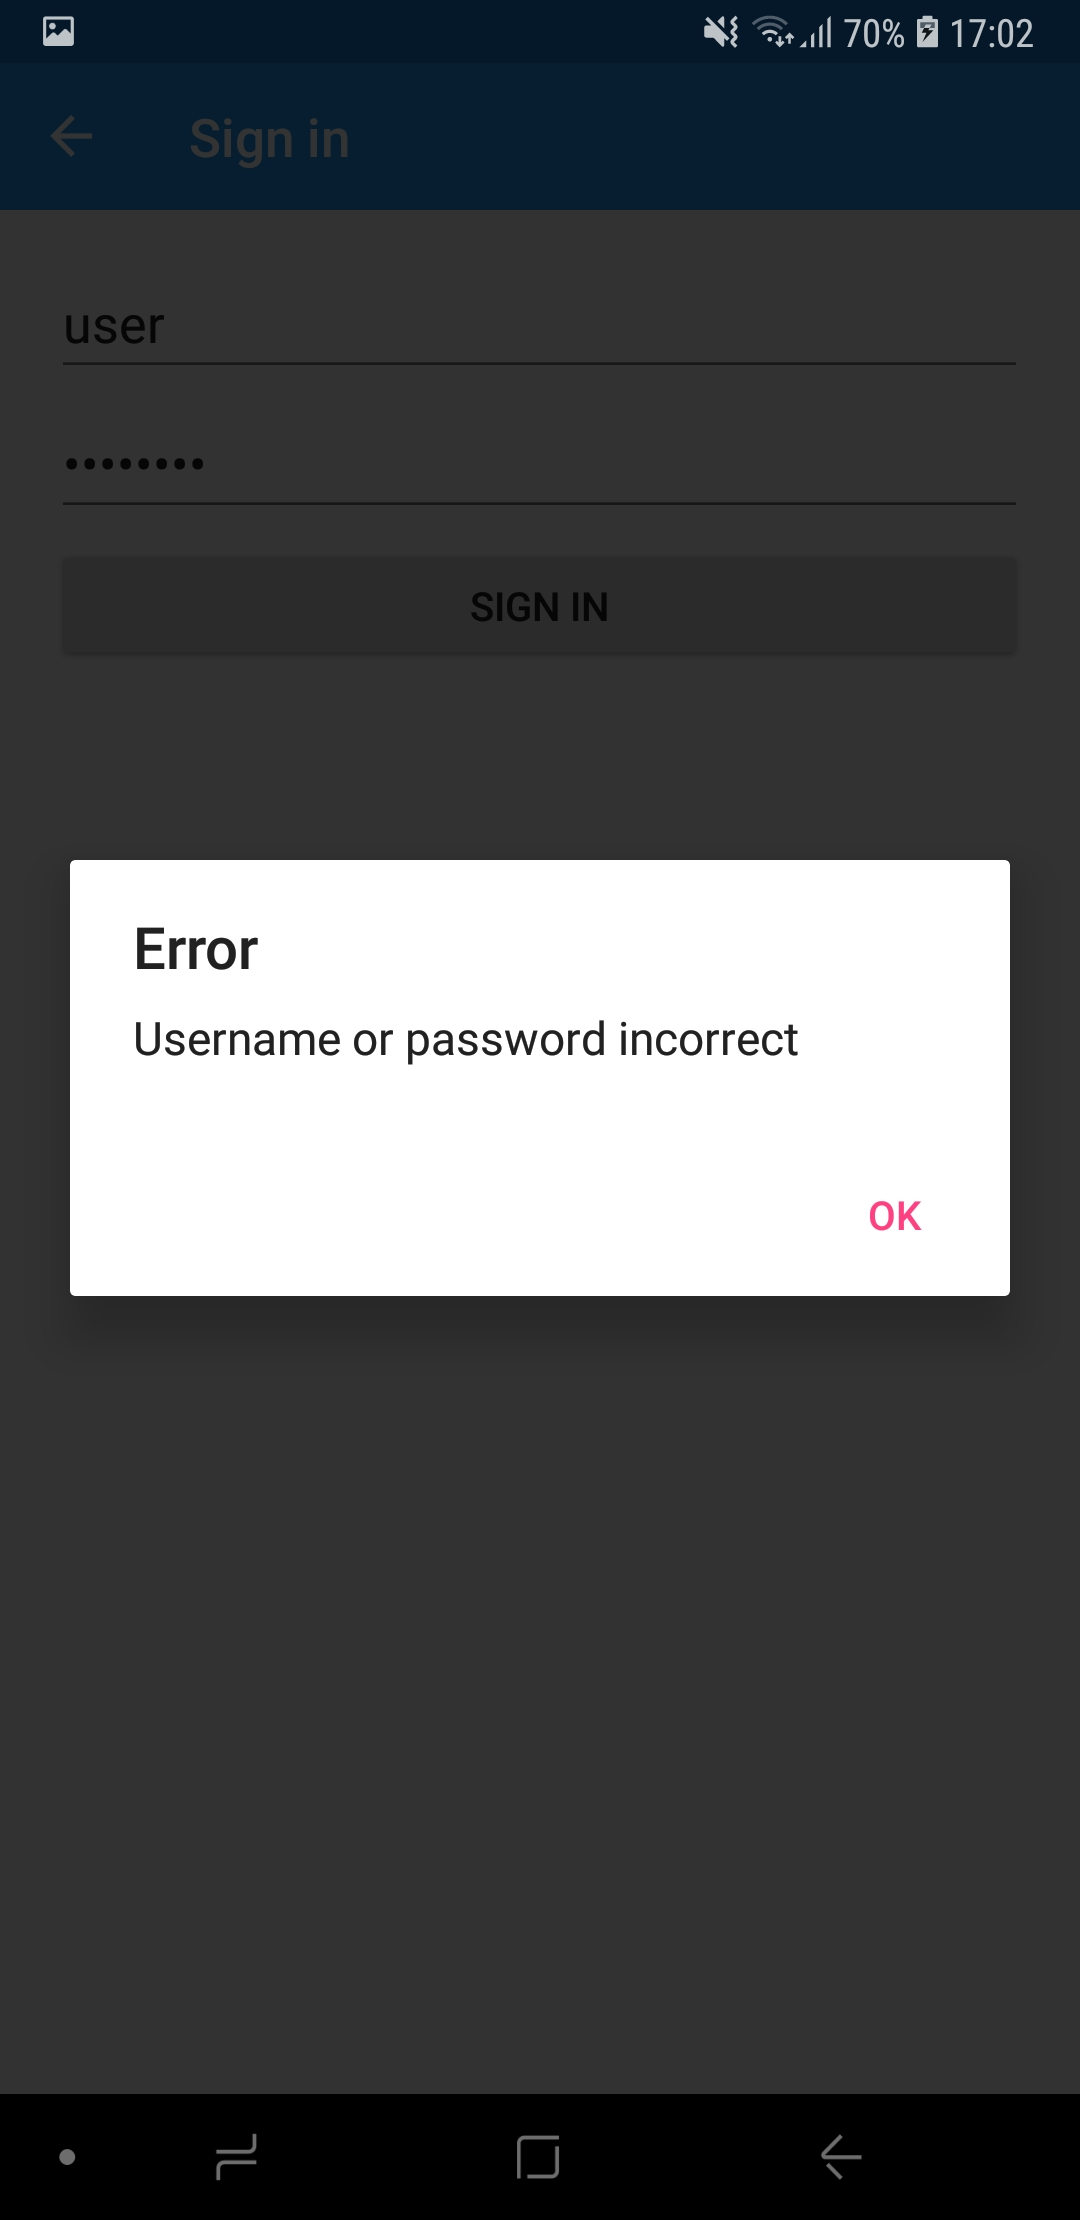
\includegraphics[width=1.75in]{img/mobile/logowanie_haslo.jpg}
			\subcaption{Błędne hasło.}
			\label{logowanie_haslo}
		\end{subfigure}
	\end{center}
	\caption{Zrzuty ekranu procesu logowania.}
\end{figure}

\textbf{Wyświetlanie danych użytkownika} (przypadek użycia "wyświetl swoje dane") - pobranie danych użytkownika i wyświetlenie ich użytkownikowi. Po uwierzytelnieniu się w aplikacji i wybraniu z menu bocznego strony "User details" (Rys. \ref{hamburger_uzytkownik}) użytkownikowi prezentowane są jego dane (Rys \ref{uzytkownik}).
\begin{figure}[!ht]
	\begin{center}
		\begin{subfigure}[b]{0.3\textwidth}
			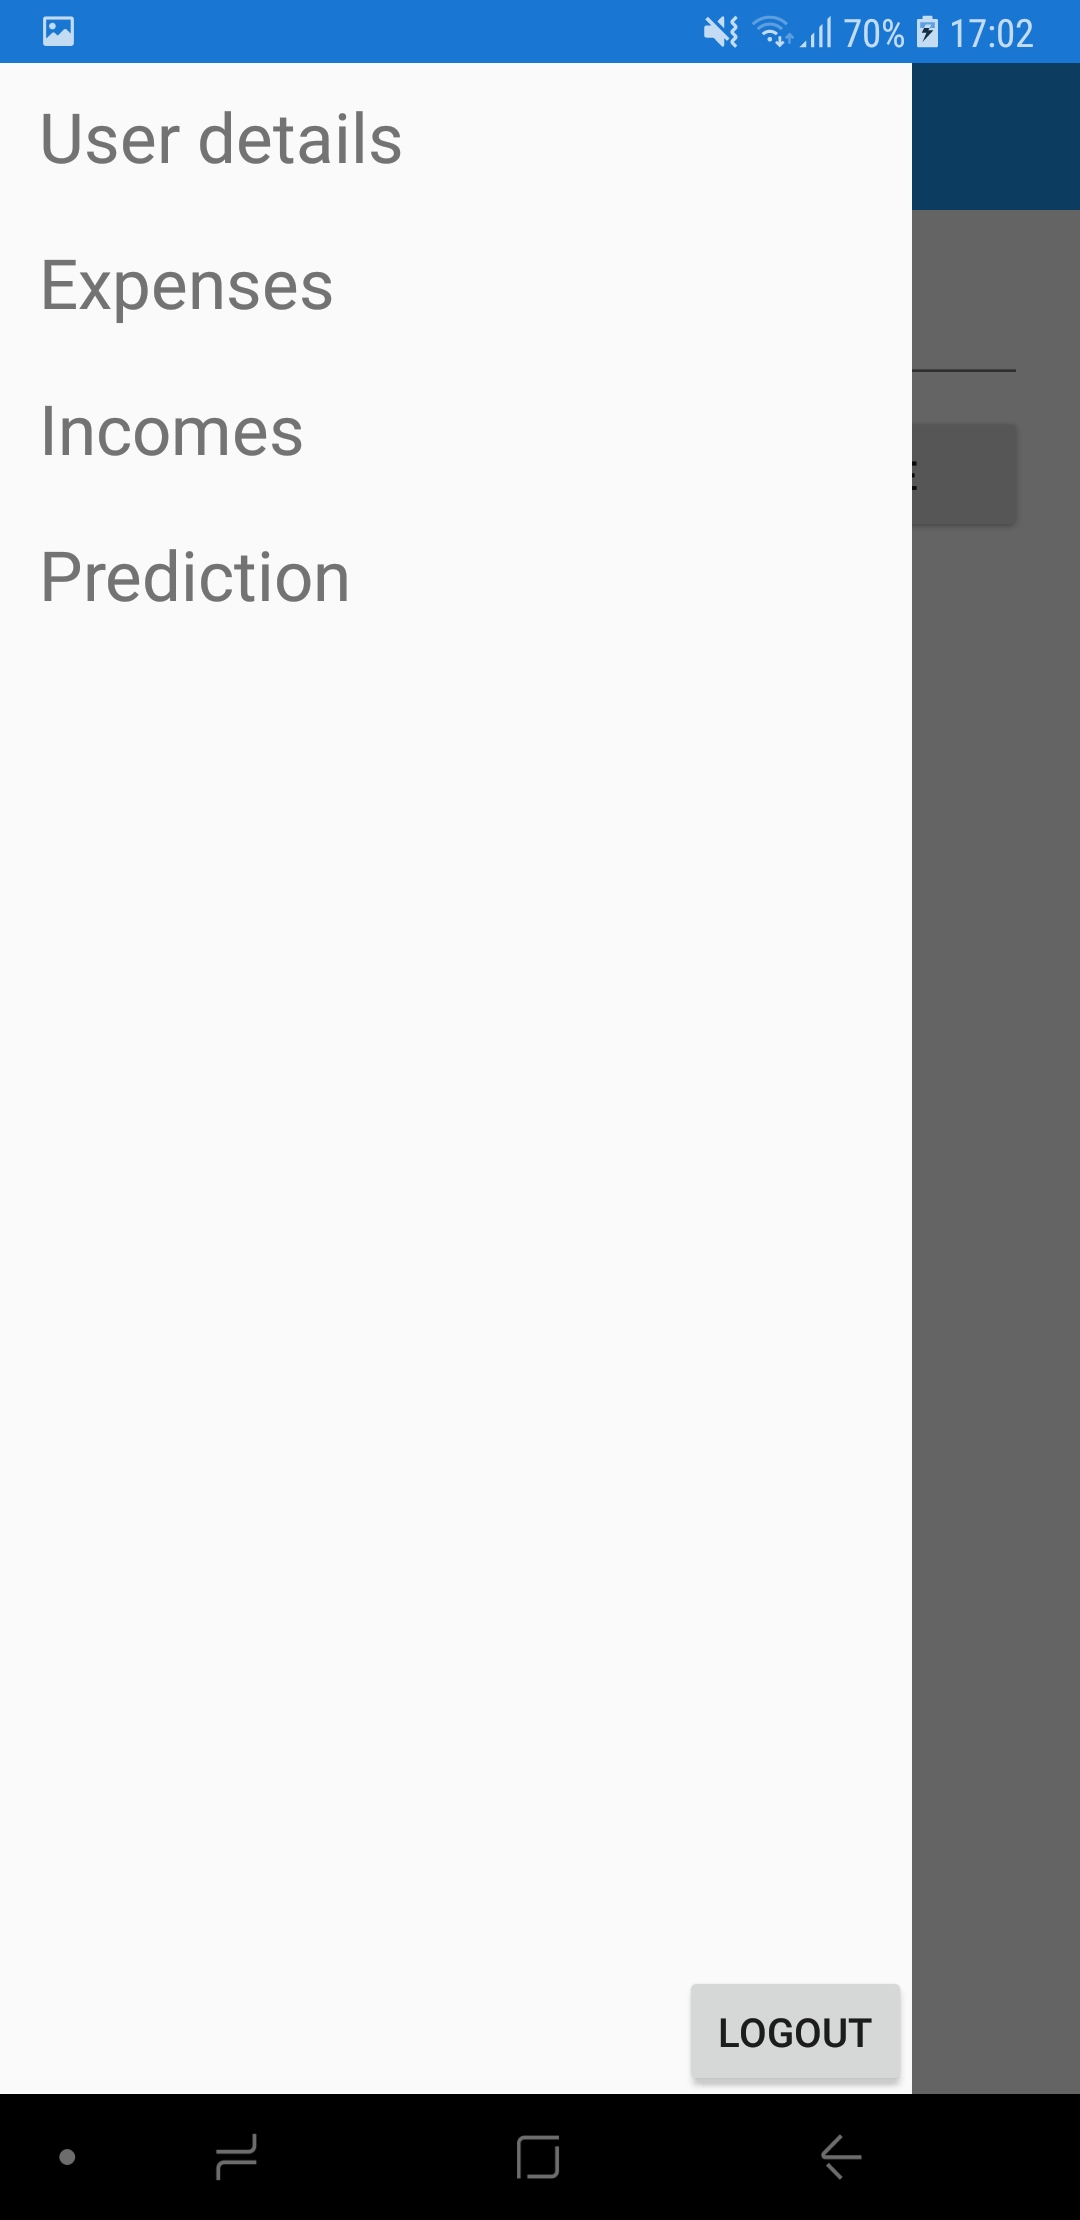
\includegraphics[width=1.75in]{img/mobile/menu_boczne.jpg}
			\subcaption{Menu boczne.}
			\label{hamburger_uzytkownik}
		\end{subfigure}
		\begin{subfigure}[b]{0.3\textwidth}
			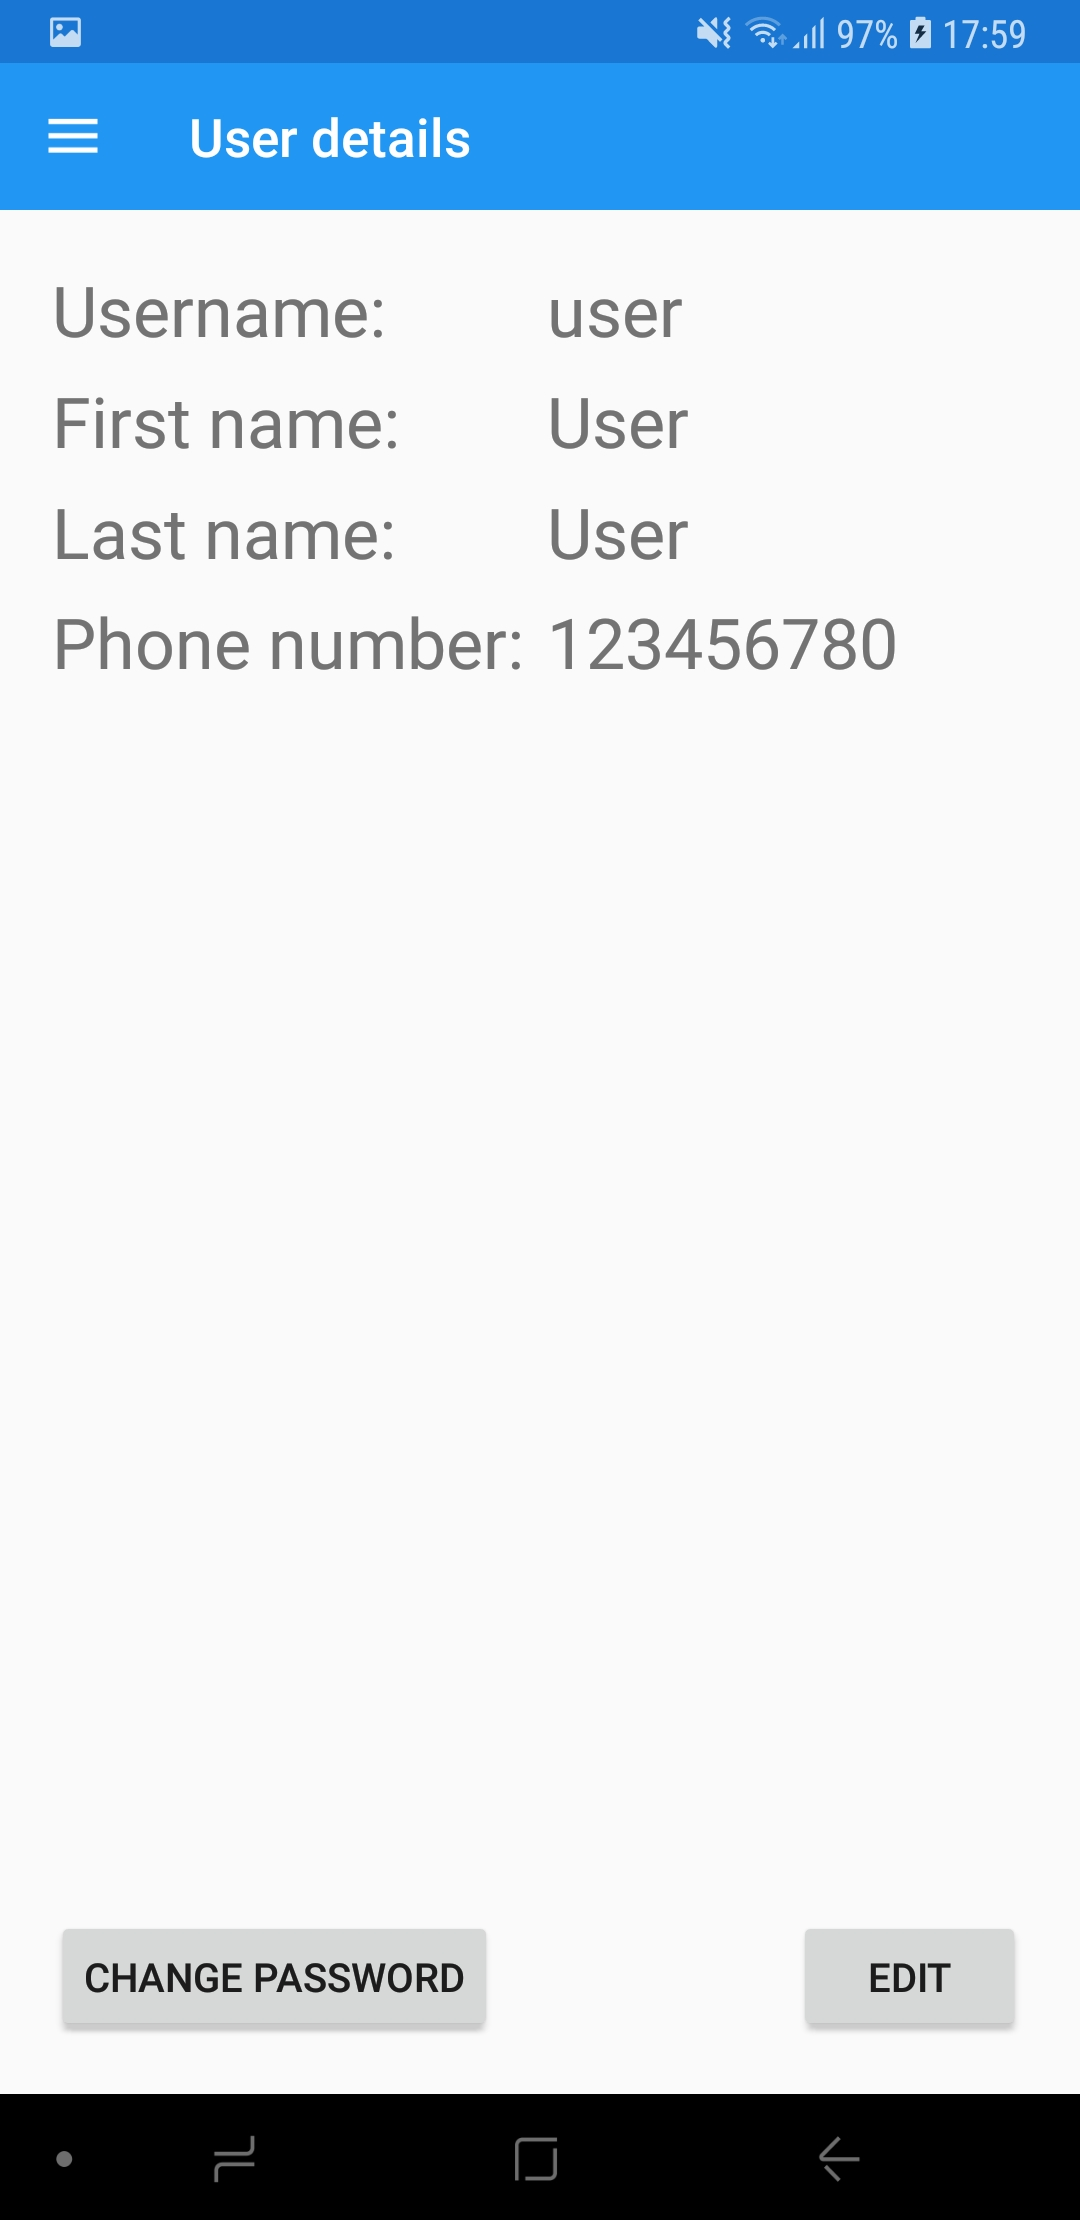
\includegraphics[width=1.75in]{img/mobile/uzytkownik.jpg}
			\subcaption{Dane użytkownika.}
			\label{uzytkownik}
		\end{subfigure}
	\end{center}
	\caption{Zrzuty ekranu procesu wyświetlania danych użytkownika.}
\end{figure}

\textbf{Edycja danych użytkownika} (przypadek użycia "edytuj swoje dane") - zmiana imienia, nazwiska bądź numeru telefonu użytkownika. Po przejściu na ekran danych użytkownika i wybraniu przycisku "EDIT" (Rys. \ref{uzytkownik_edit}) otwierany jest formularz edycji (Rys. \ref{edycja_uzytkownika}). Wciśnięcie przycisku "SUBMIT" edytuje dane użytkownika, przycisk "BACK" odrzuca wszelkie wprowadzone zmiany.
\begin{figure}[!ht]
	\begin{center}
		\begin{subfigure}[b]{0.3\textwidth}
			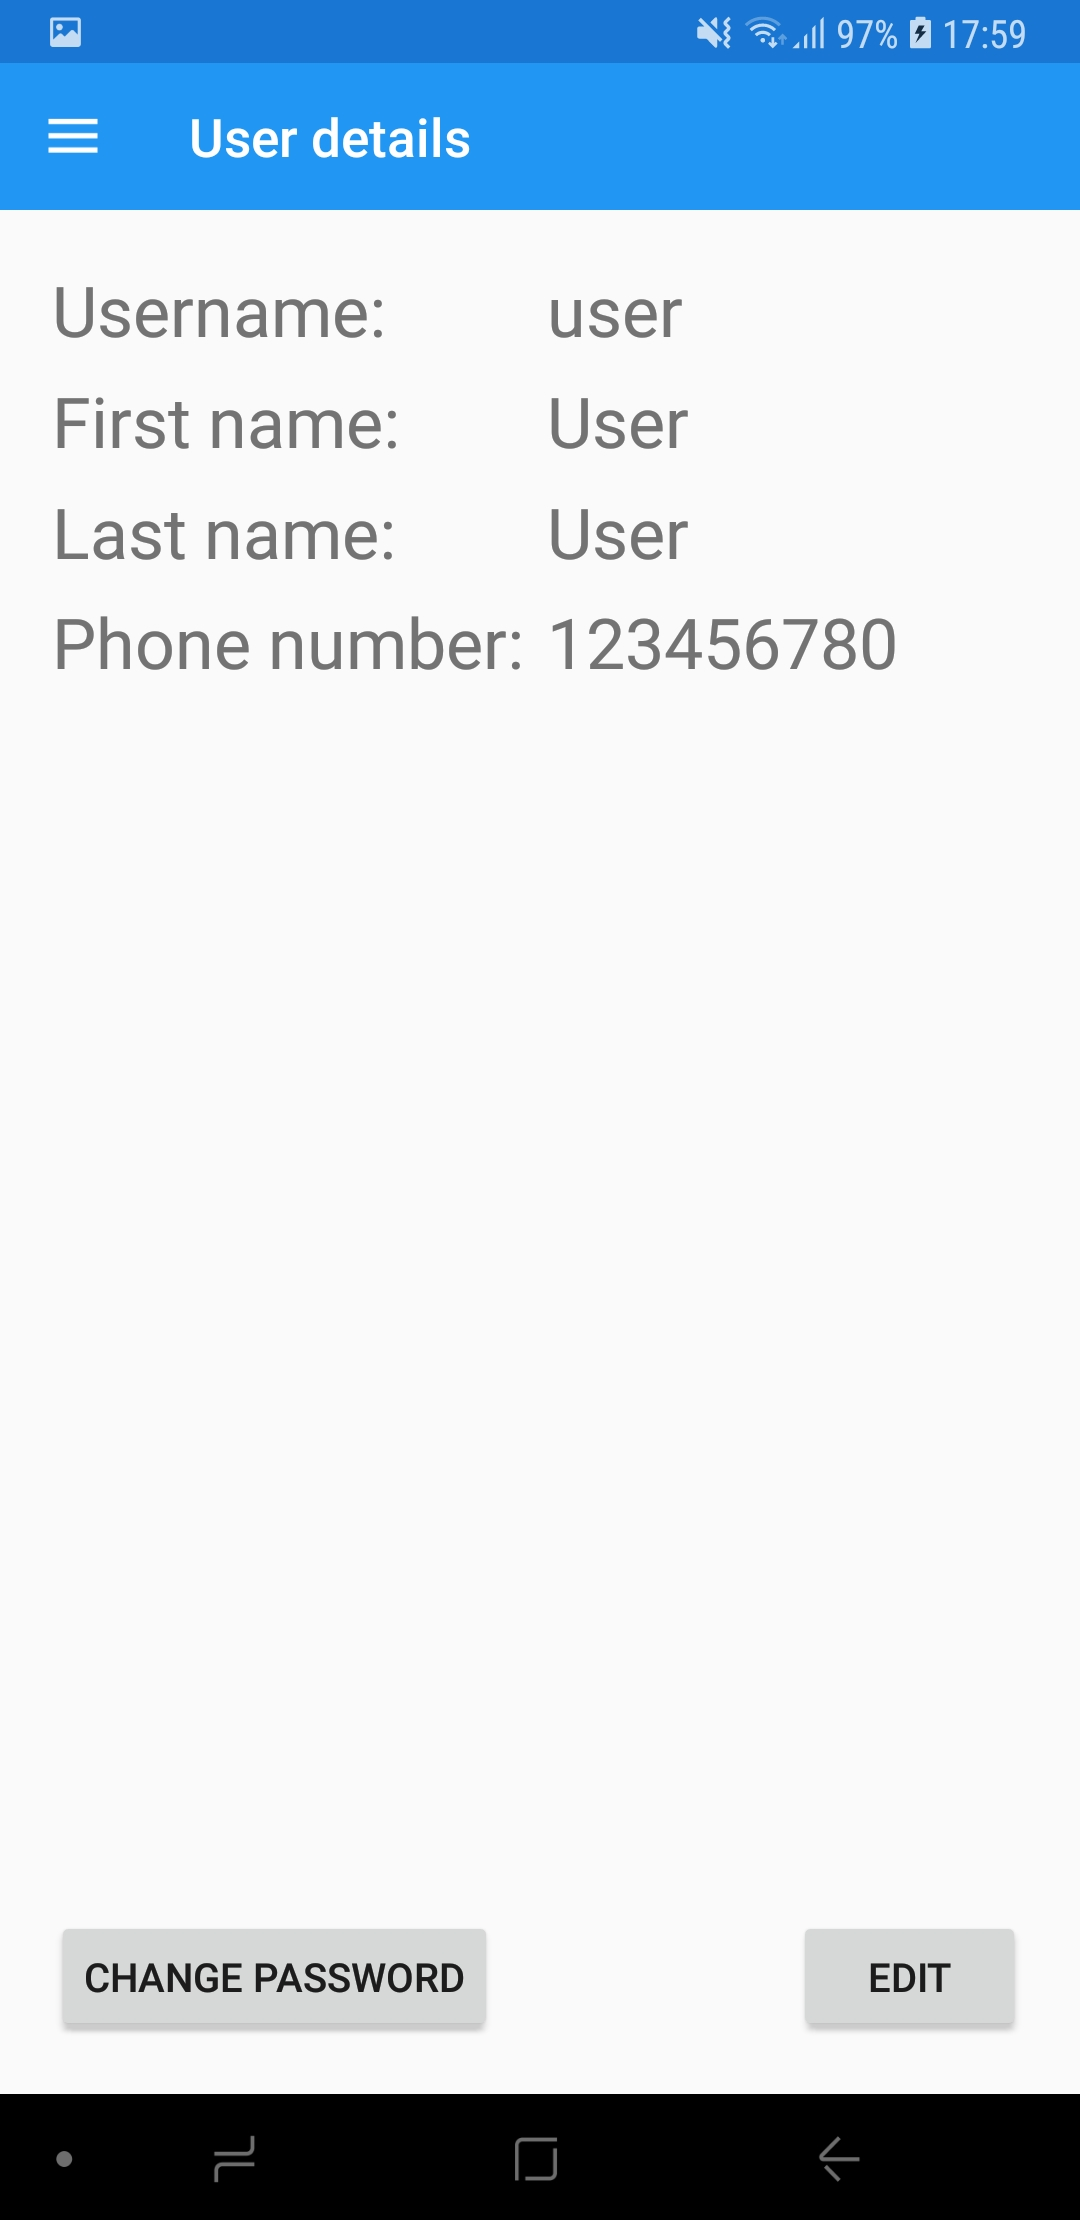
\includegraphics[width=1.75in]{img/mobile/uzytkownik.jpg}
			\subcaption{Dane użytkownika.\newline}
			\label{uzytkownik_edit}
		\end{subfigure}
		\begin{subfigure}[b]{0.3\textwidth}
			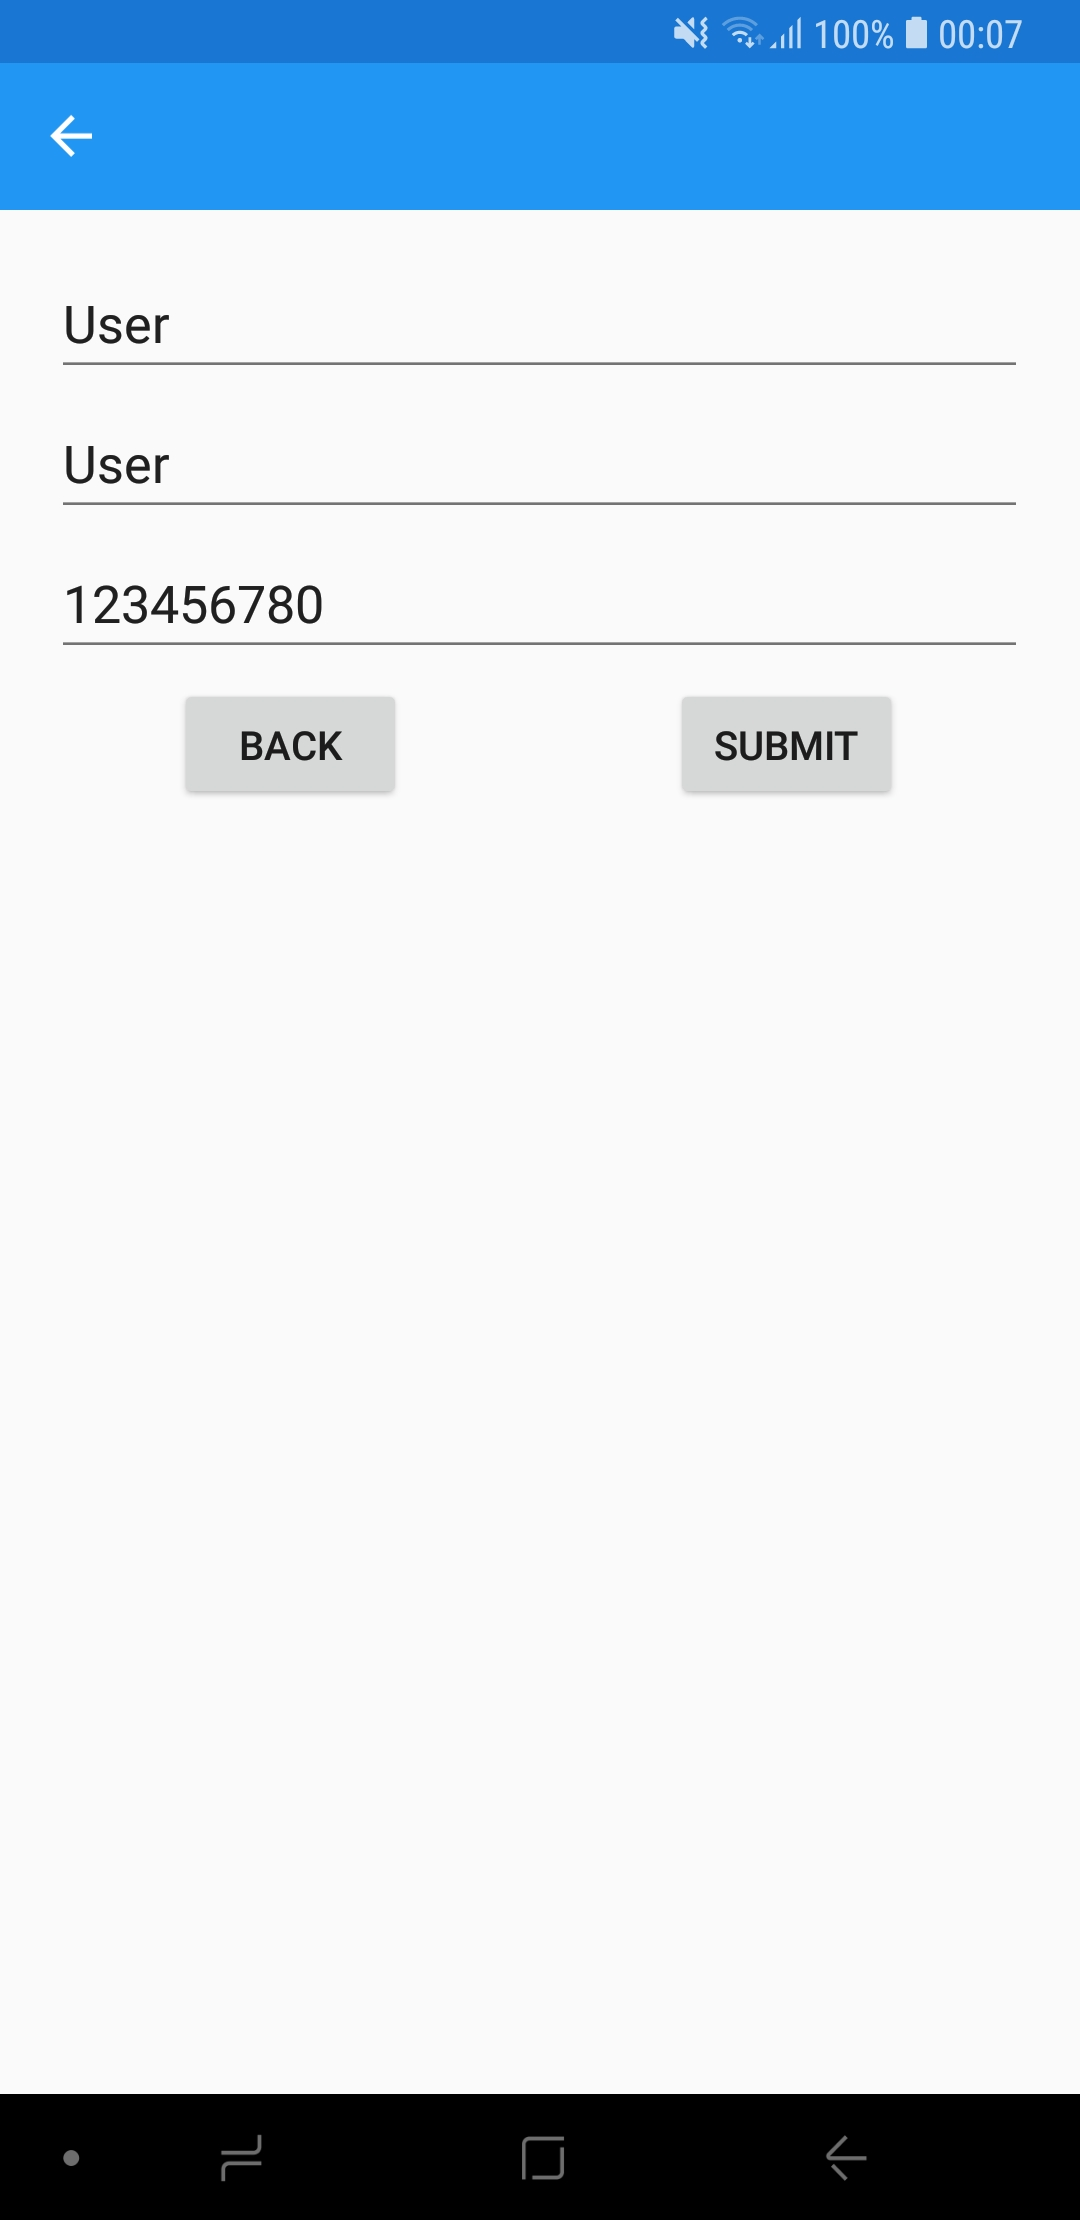
\includegraphics[width=1.75in]{img/mobile/edycja_uzytkownika.jpg}
			\subcaption{Edycja danych użytkownika.}
			\label{edycja_uzytkownika}
		\end{subfigure}
	\end{center}
	\caption{Zrzuty ekranu procesu edycji danych użytkownika.}
\end{figure}

\textbf{Zmiana hasła} (przypadek użycia "zmień swoje hasło) - ustawienie nowego hasła użytkownika. Po wybraniu przycisku "CHANGE PASSWORD" na ekranie danych użytkownika (Rys. \ref{uzytkownik_pass}) wyświetlany jest formularz zmiany hasła (Rys. \ref{haslo}). Poprawne wypełnienie formularza i naciśnięcie przycisku "SUBMIT" skutkuje zmianą hasła lub, jeżeli nie spełnia ono polityki haseł, wyświetlany jest komunikat o błędzie (Rys. \ref{haslo_blad}). Wciśnięcie przycisku "BACK" powoduje powrót do strony danych użytkownika.
\begin{figure}[!ht]
	\begin{center}
		\begin{subfigure}[b]{0.3\textwidth}
			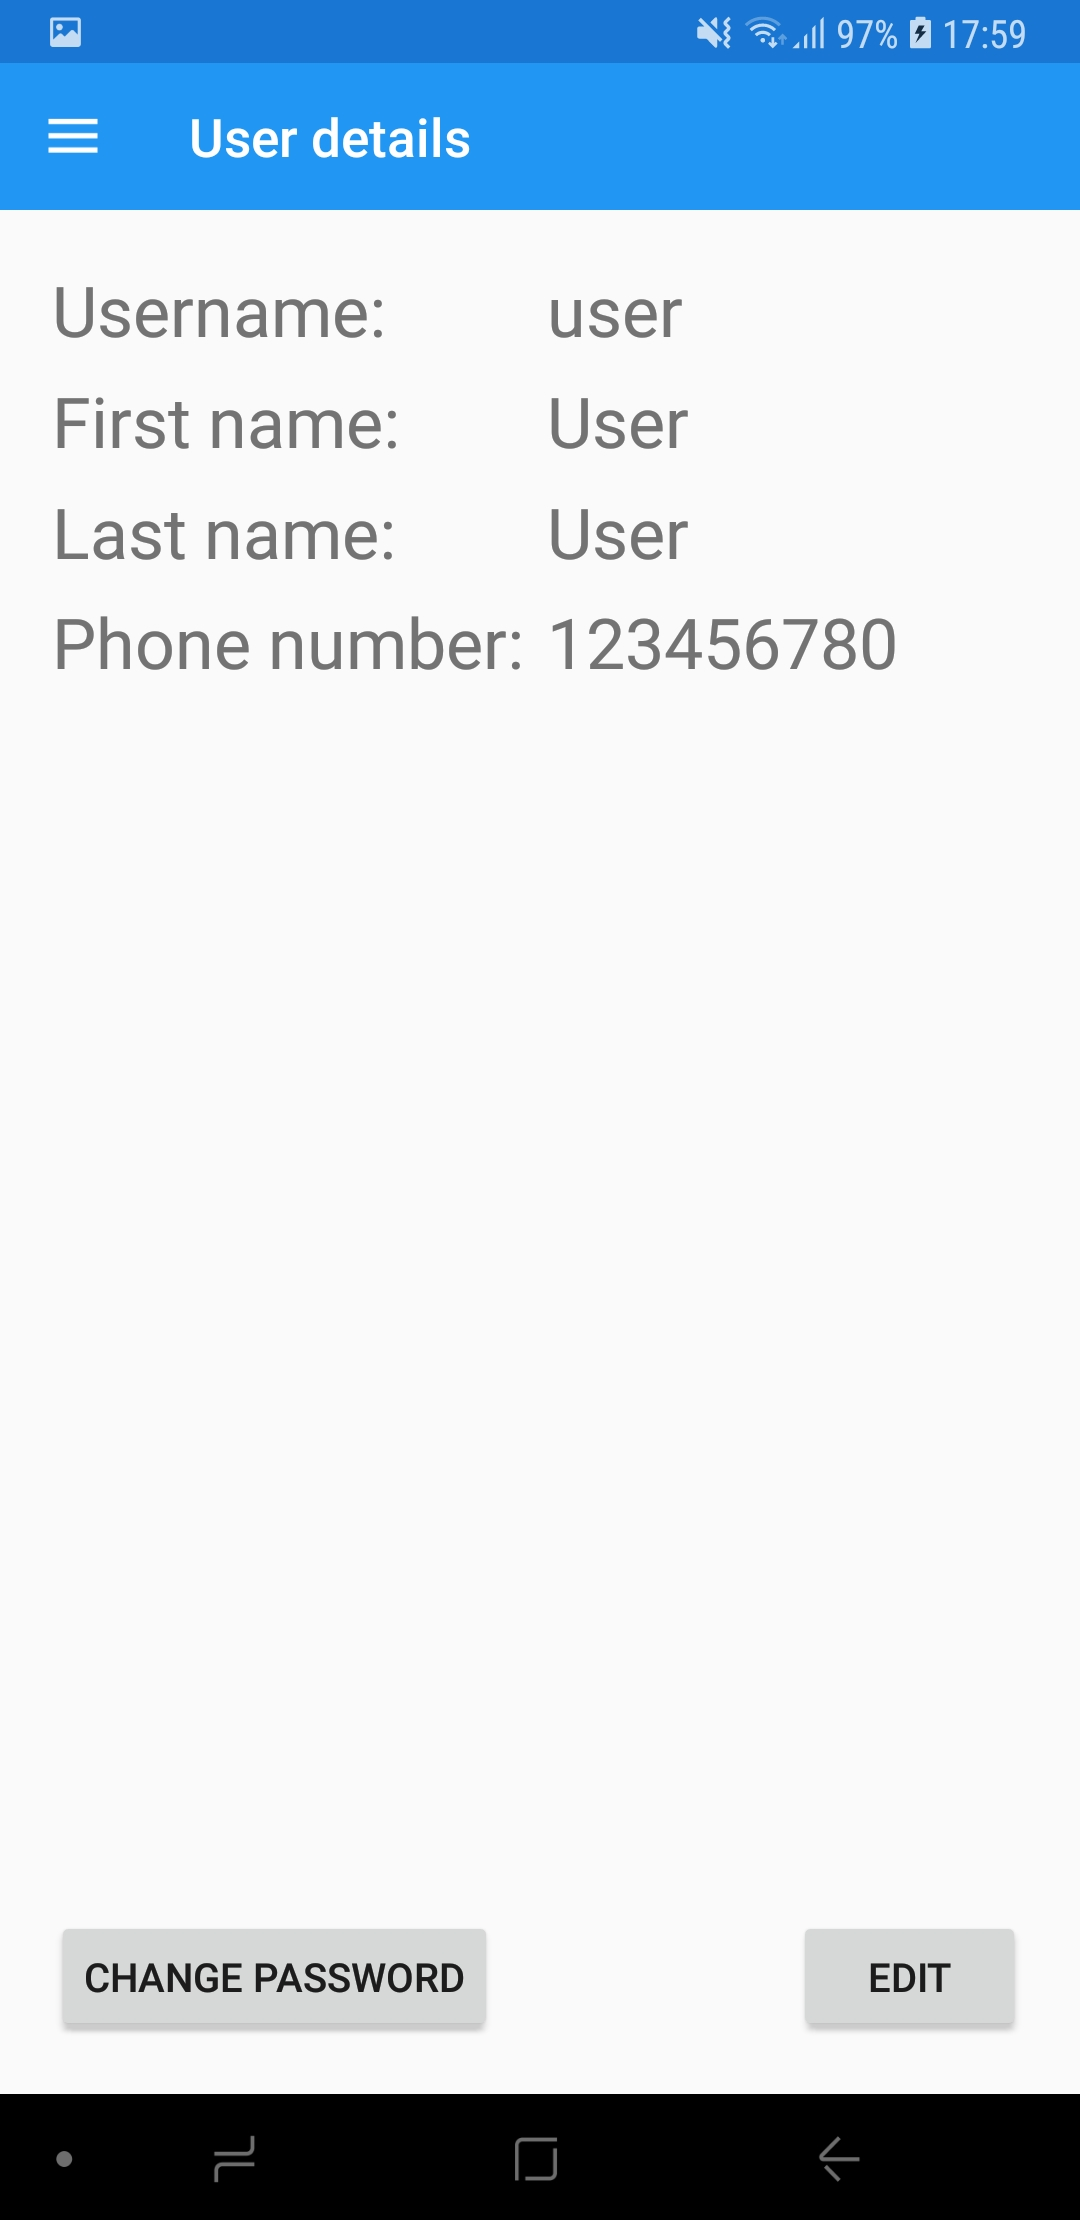
\includegraphics[width=1.75in]{img/mobile/uzytkownik.jpg}
			\subcaption{Dane użytkownika.}
			\label{uzytkownik_pass}
		\end{subfigure}
		\begin{subfigure}[b]{0.3\textwidth}
			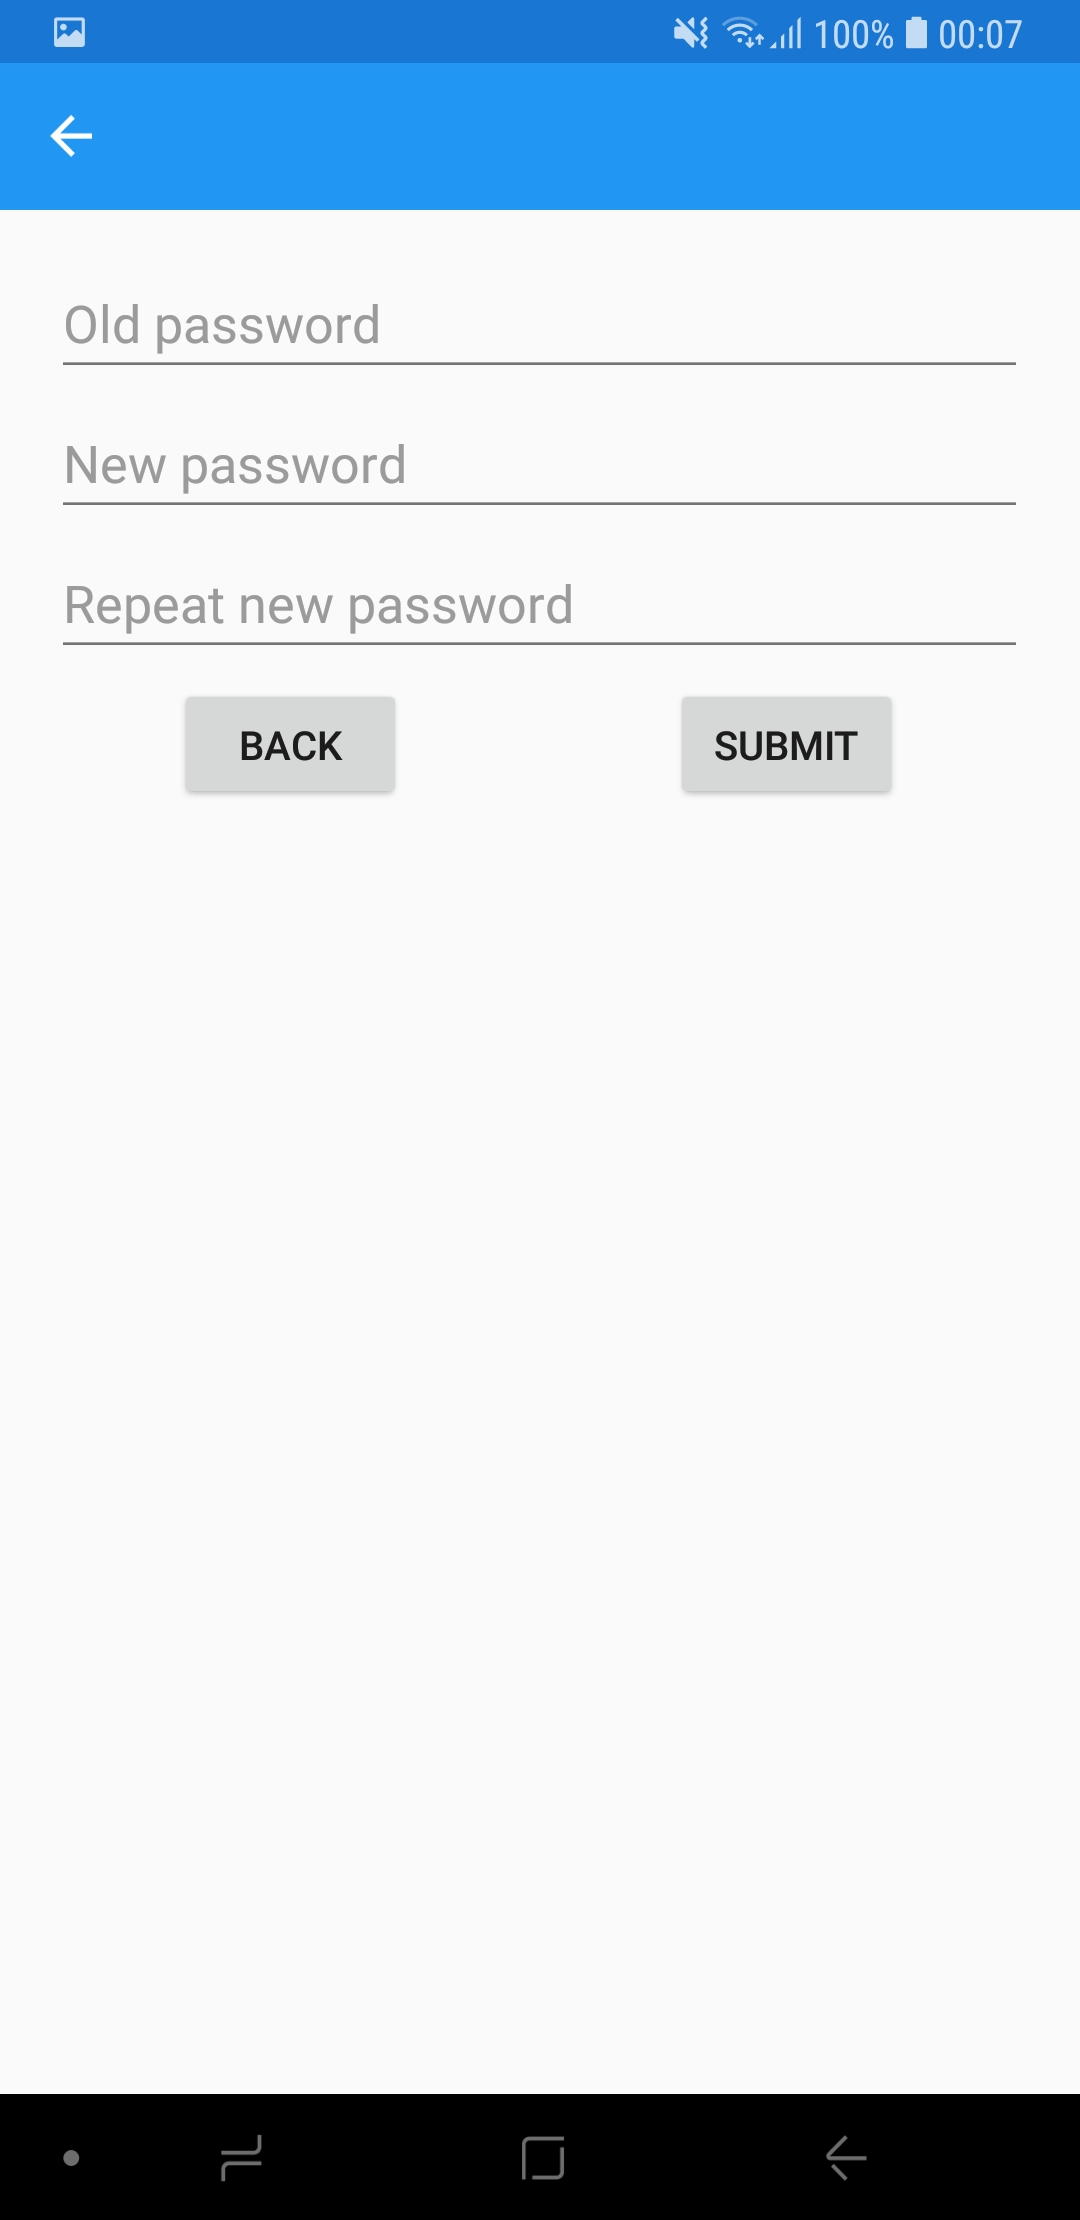
\includegraphics[width=1.75in]{img/mobile/haslo.jpg}
			\subcaption{Formularz zmiany hasła.}
			\label{haslo}
		\end{subfigure}
		\begin{subfigure}[b]{0.3\textwidth}
			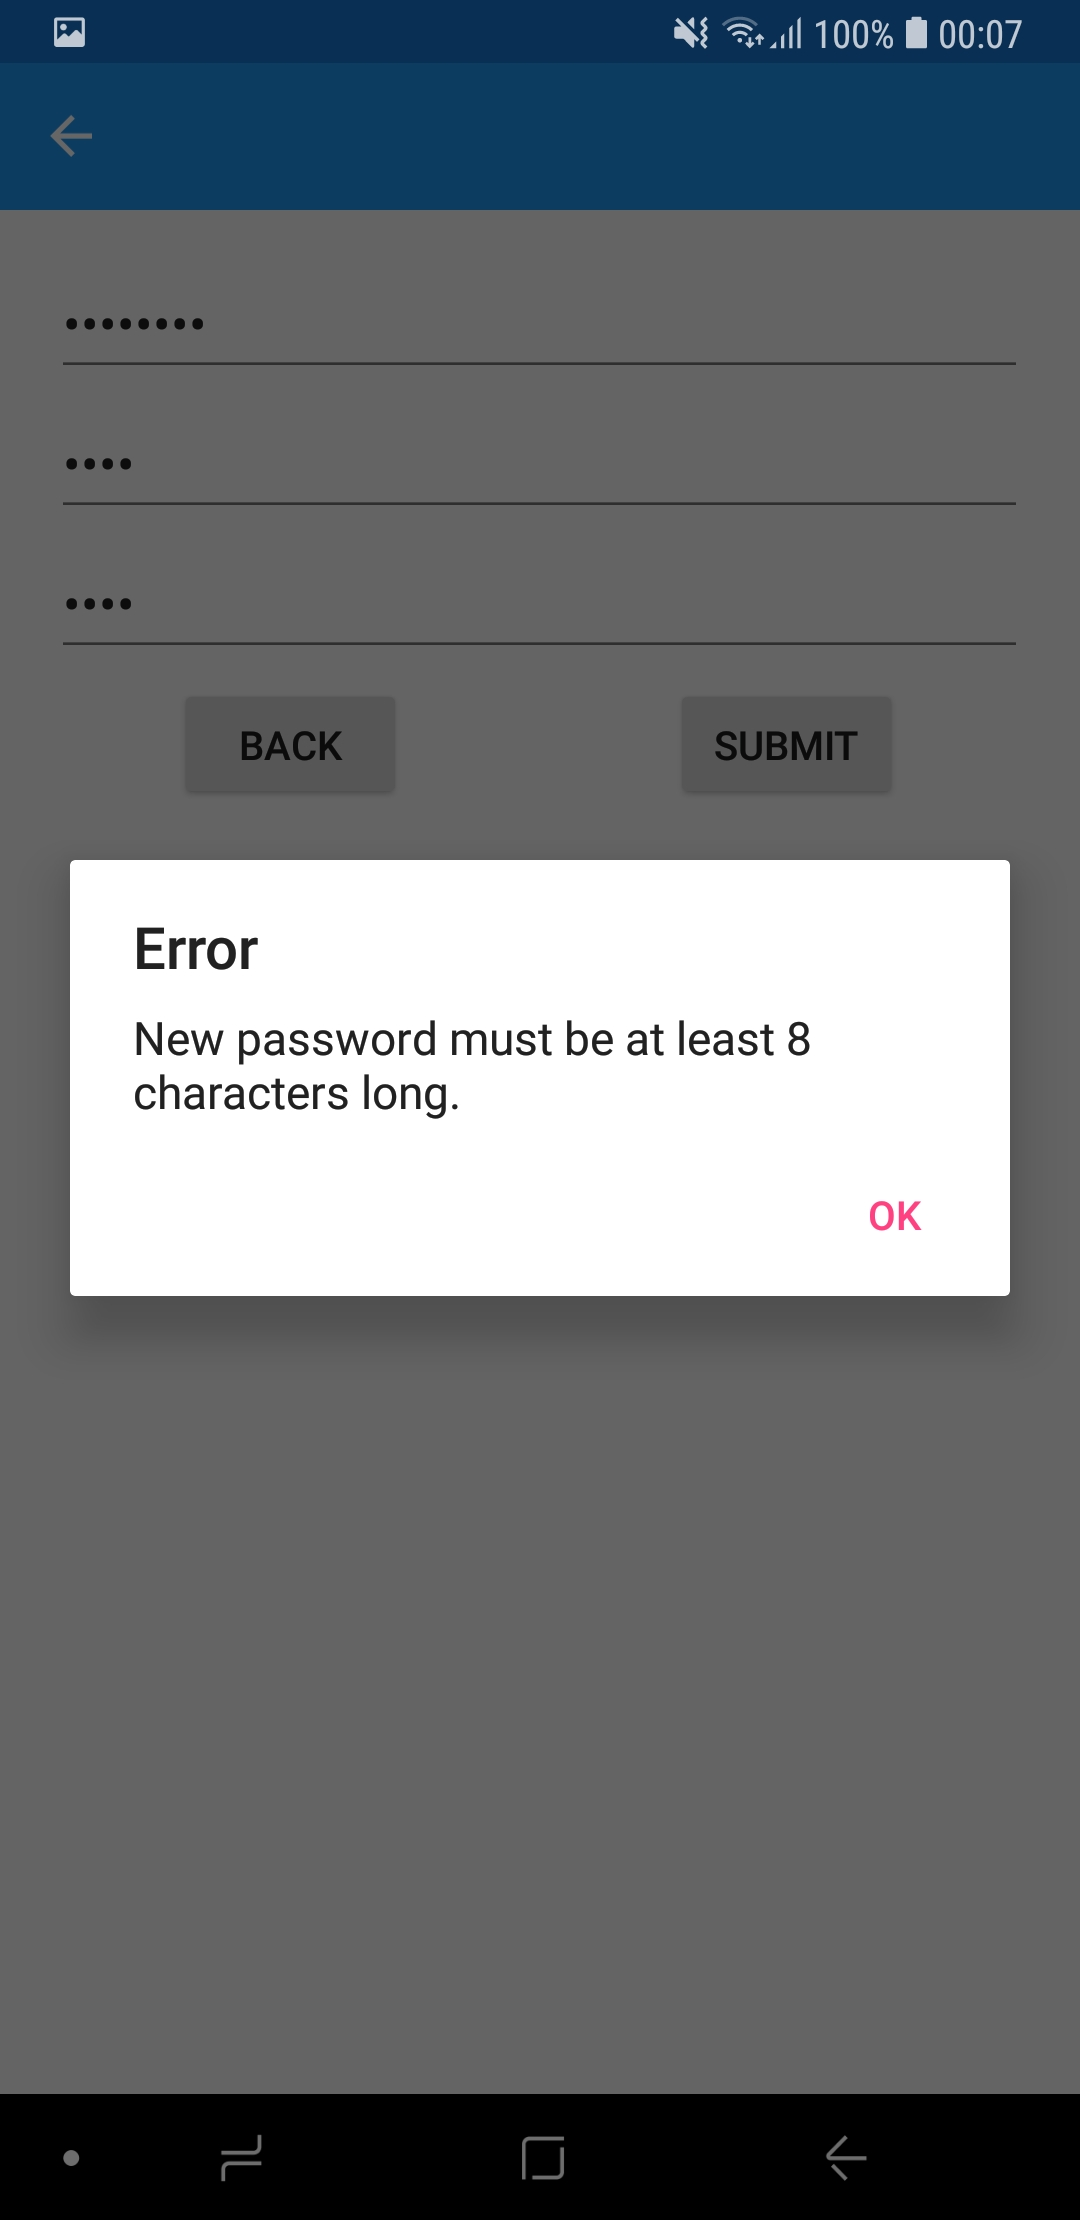
\includegraphics[width=1.75in]{img/mobile/haslo_blad.jpg}
			\subcaption{Komunikat o błędzie.}
			\label{haslo_blad}
		\end{subfigure}
	\end{center}
	\caption{Zrzuty ekranu procesu zmiany hasła.}
\end{figure}
\section{Moduł rejestracji przychodów}
Moduł rejestracji przychodów składa się z czterech przypadków użycia:
\begin{itemize}
\item wyświetl swoje przychody,
\item dodaj przychód,
\item edytuj przychód,
\item usuń przychód.
\end{itemize}

\textbf{Wyświetlanie przychodów} (przypadek użycia "wyświetl swoje przychody") - pobranie i zaprezentowanie użytkownikowi listy jego przychodów z danego okresu. Po wybraniu z menu bocznego (Rys. \ref{hamburger_przychody}) strony "Incomes" (Rys. \ref{przychody}), określeniu daty początkowej i końcowej oraz naciśnięciu przycisku "GET INCOMES" wyświetlana jest lista przychodów z wybranego okresu (Rys. \ref{przychody_gotowe}).
\begin{figure}[!ht]
	\begin{center}
		\begin{subfigure}[b]{0.3\textwidth}
			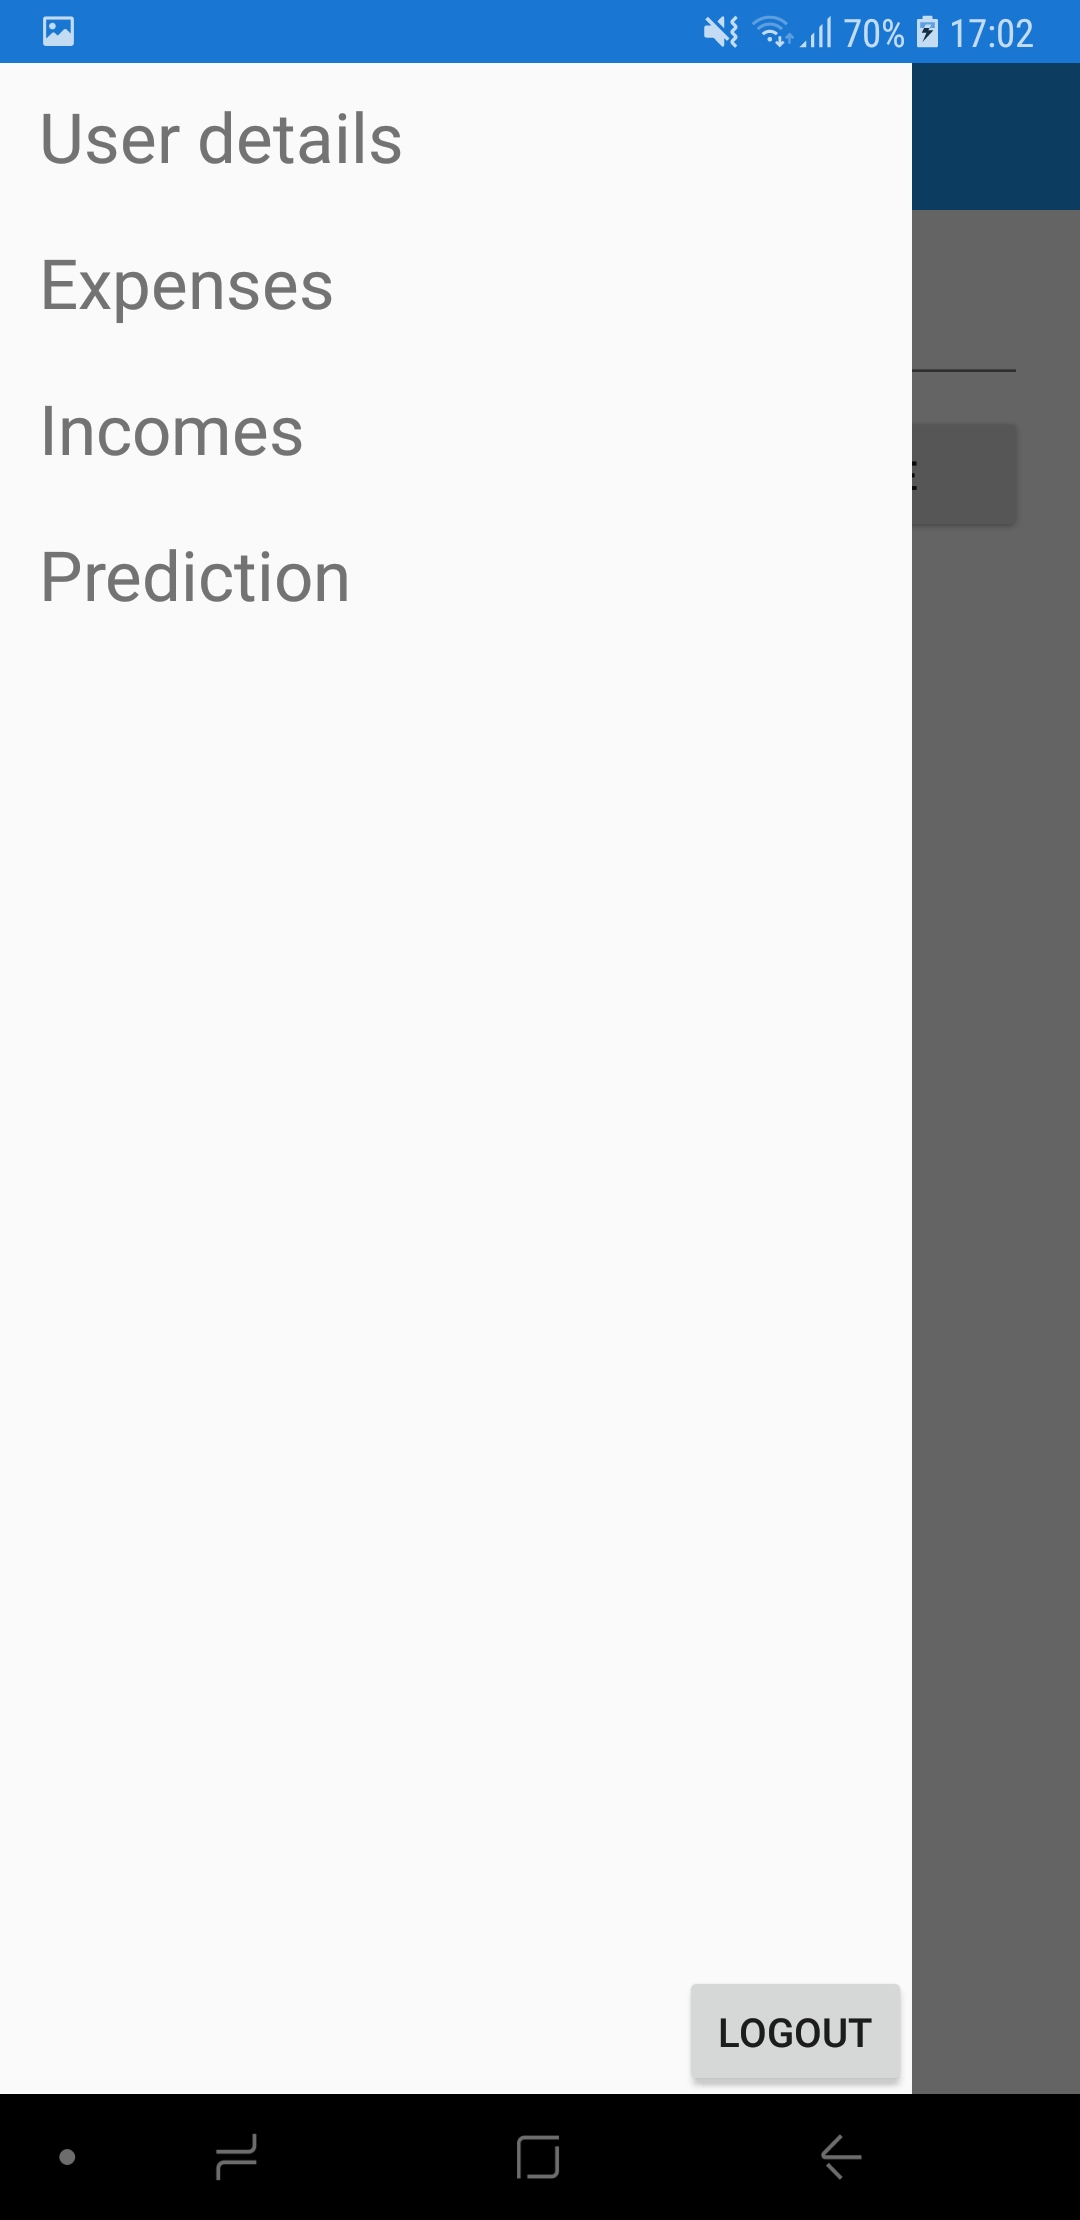
\includegraphics[width=1.75in]{img/mobile/menu_boczne.jpg}
			\subcaption{Menu boczne.}
			\label{hamburger_przychody}
		\end{subfigure}
		\begin{subfigure}[b]{0.3\textwidth}
			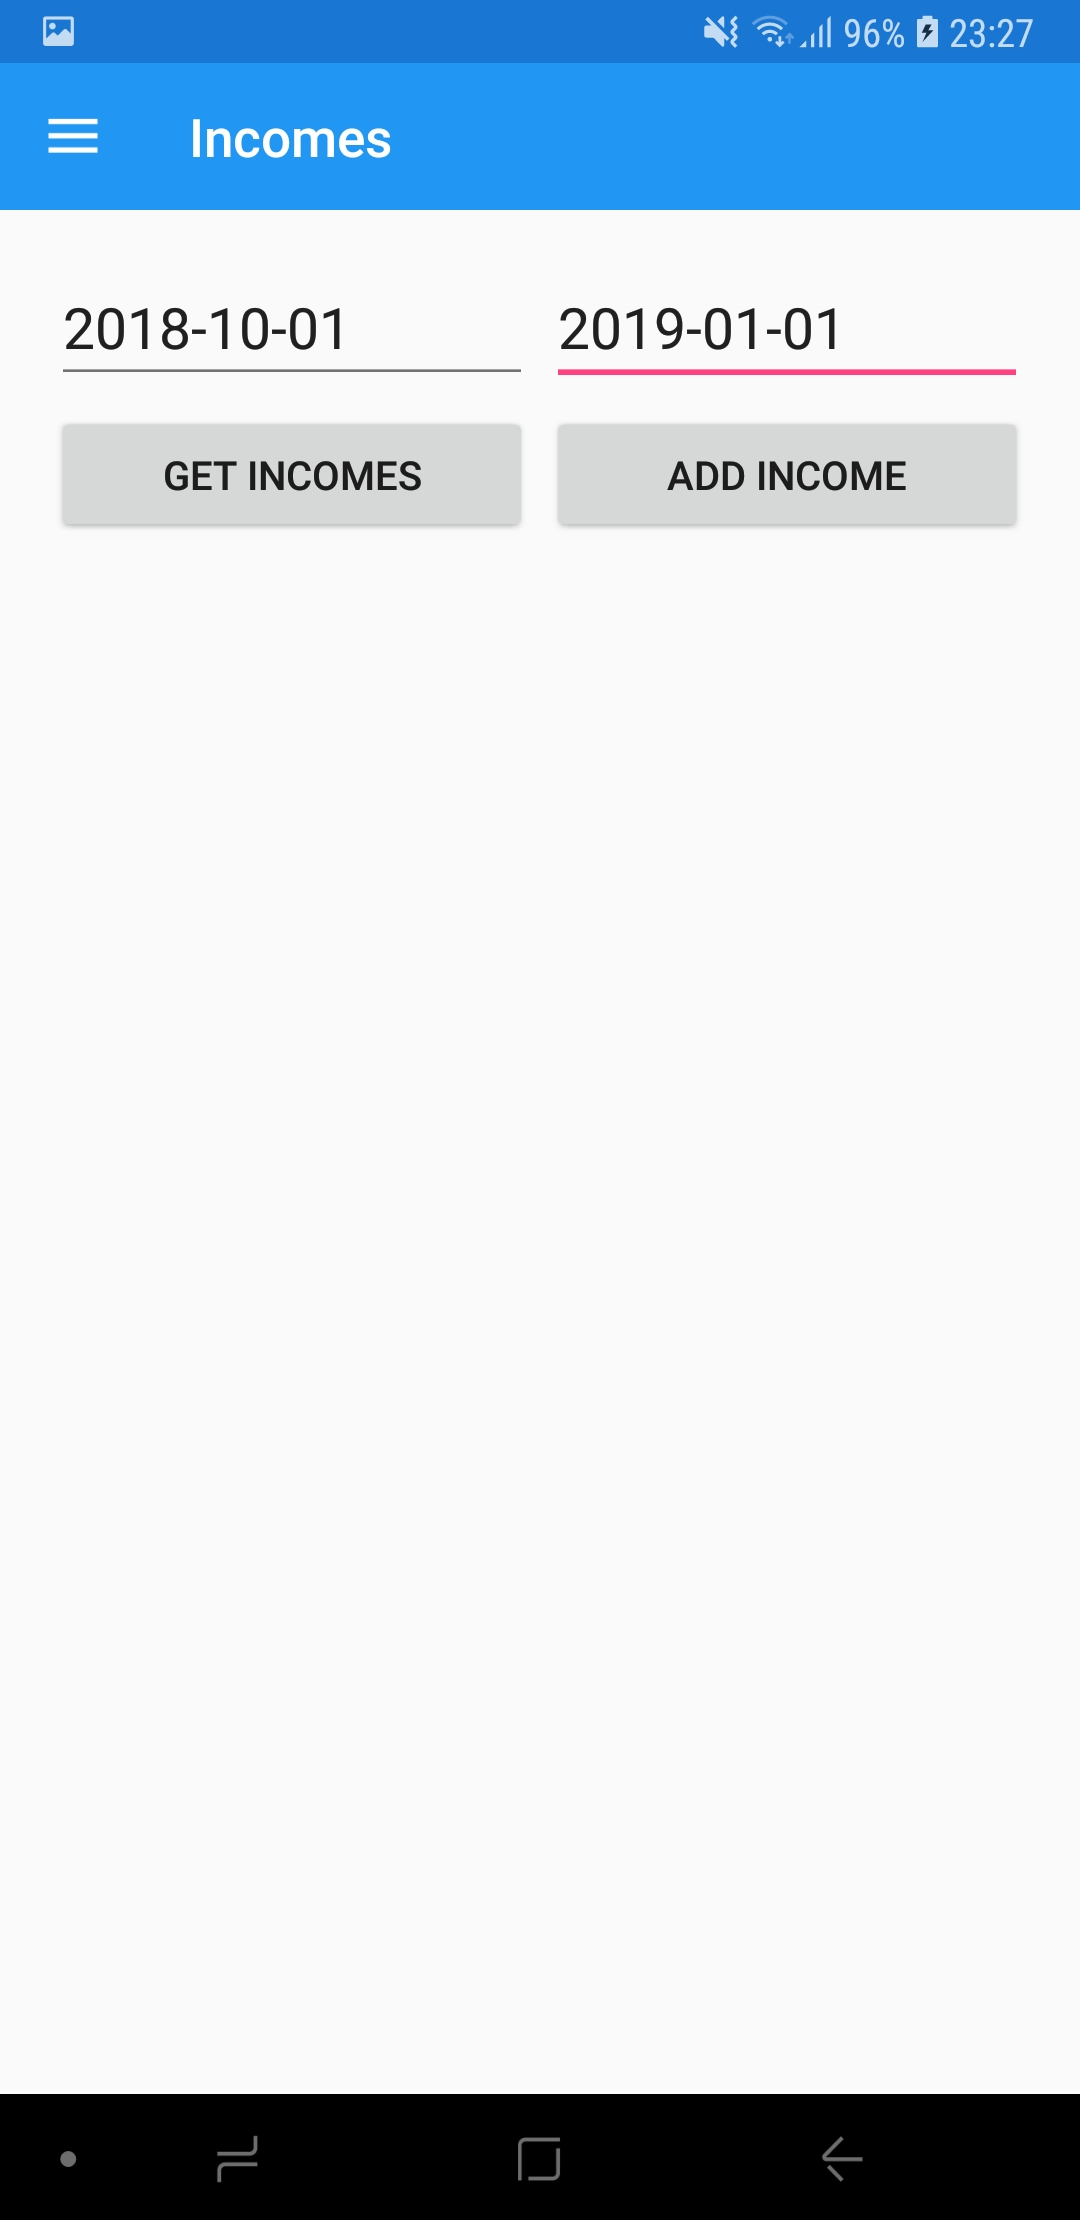
\includegraphics[width=1.75in]{img/mobile/przychody.jpg}
			\subcaption{Strona z przychodami.}
			\label{przychody}
		\end{subfigure}
		\begin{subfigure}[b]{0.3\textwidth}
			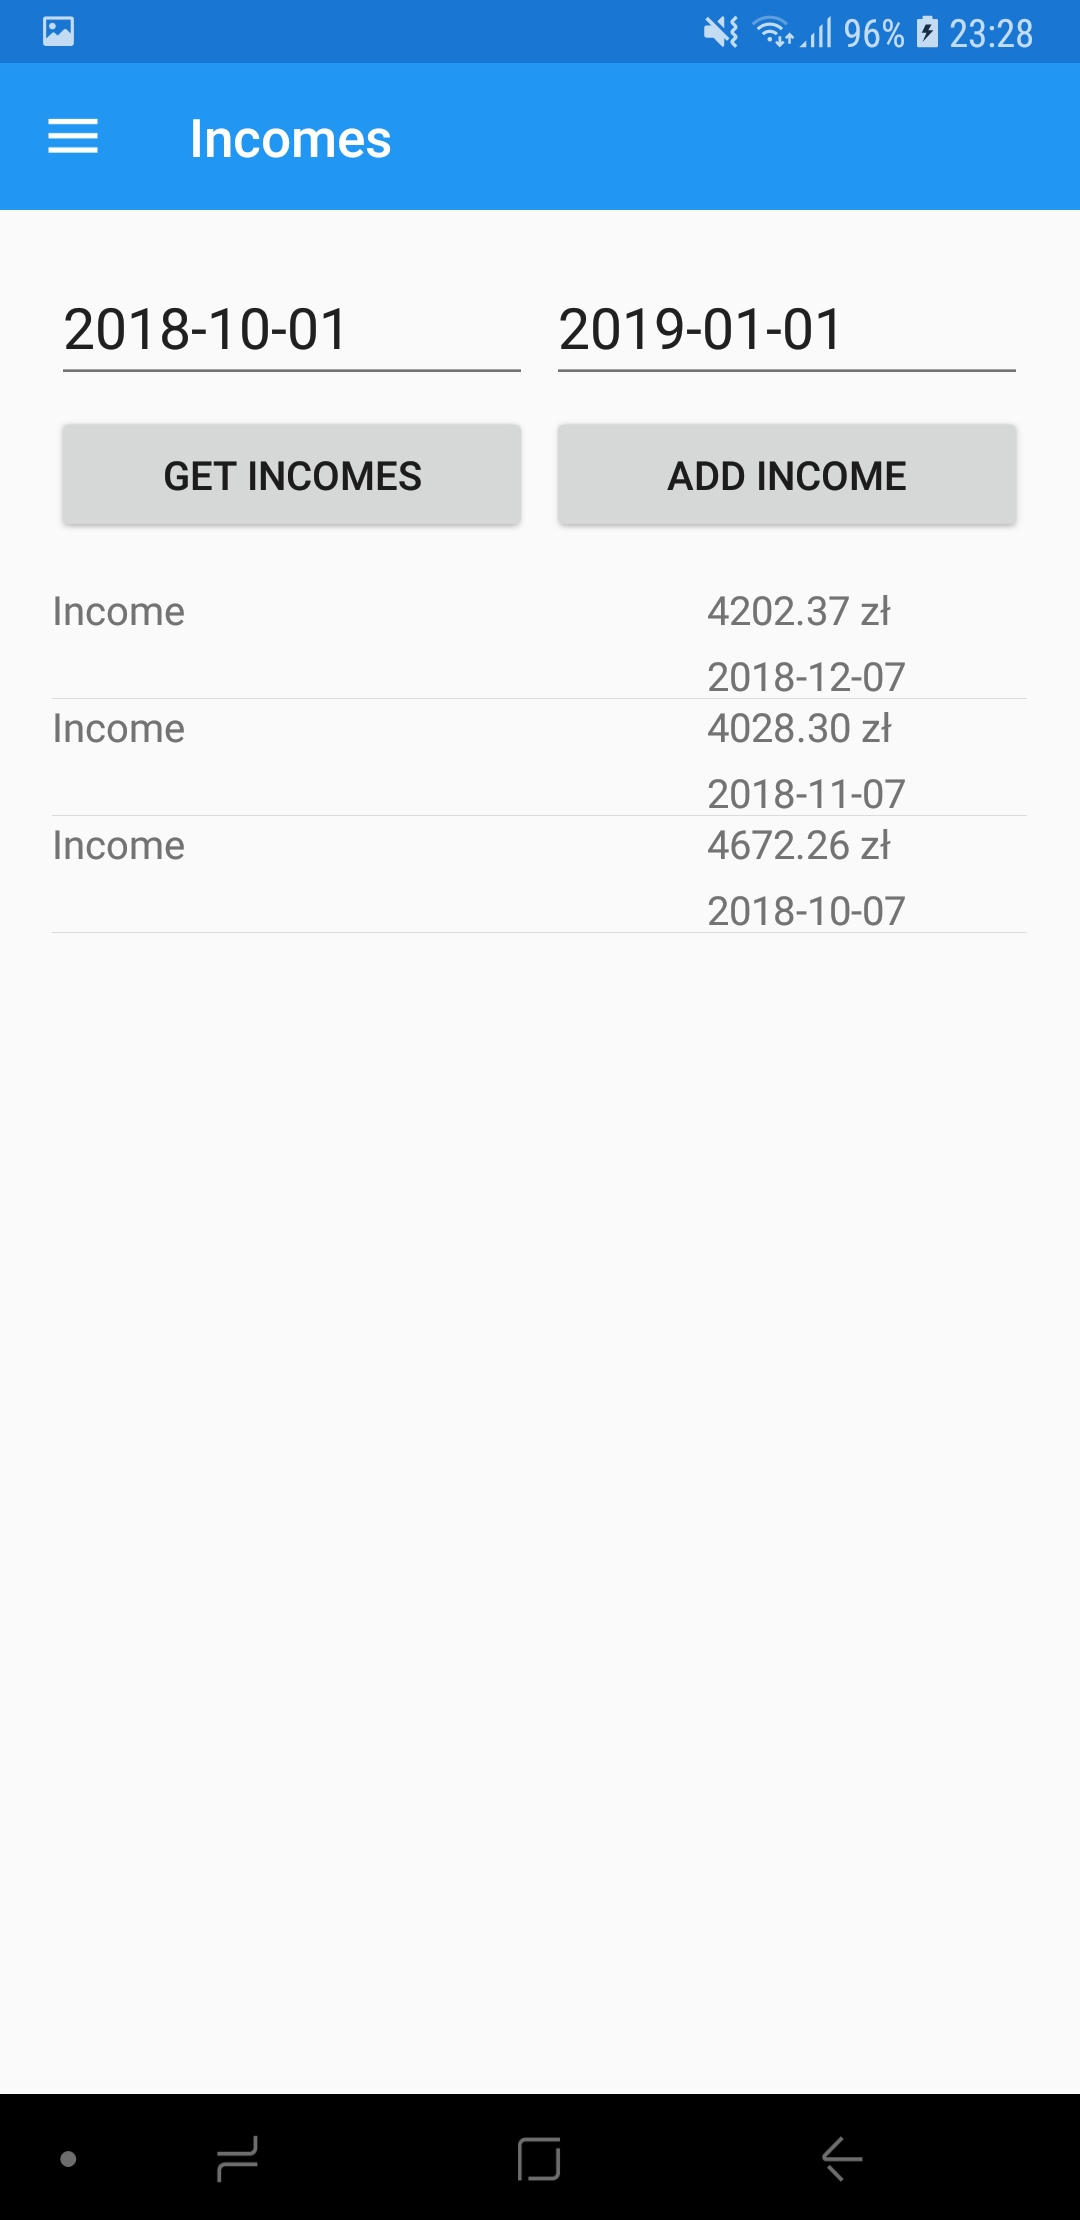
\includegraphics[width=1.75in]{img/mobile/przychody_gotowe.jpg}
			\subcaption{Lista przychodów.}
			\label{przychody_gotowe}
		\end{subfigure}
	\end{center}
	\caption{Zrzuty ekranu procesu wyświetlania przychodów.}
\end{figure}

\textbf{Dodawanie przychodu} (przypadek użycia "dodaj przychód") - dodanie wpisu z przychodem uwierzytelnionego użytkownika. Wybranie przycisku "ADD INCOME" na stronie przychodów (Rys. \ref{(przychody_dodaj}) powoduje wyświetlenie formularza dodawania przychodu (Rys. \ref{dodaj_przychod}). Po wypełnieniu formularza przy pomocy przycisku "ADD" przychód jest dodawany, a przycisk "BACK" skutkuje powrotem do strony przychodów.
\begin{figure}[!ht]
	\begin{center}
		\begin{subfigure}[b]{0.3\textwidth}
			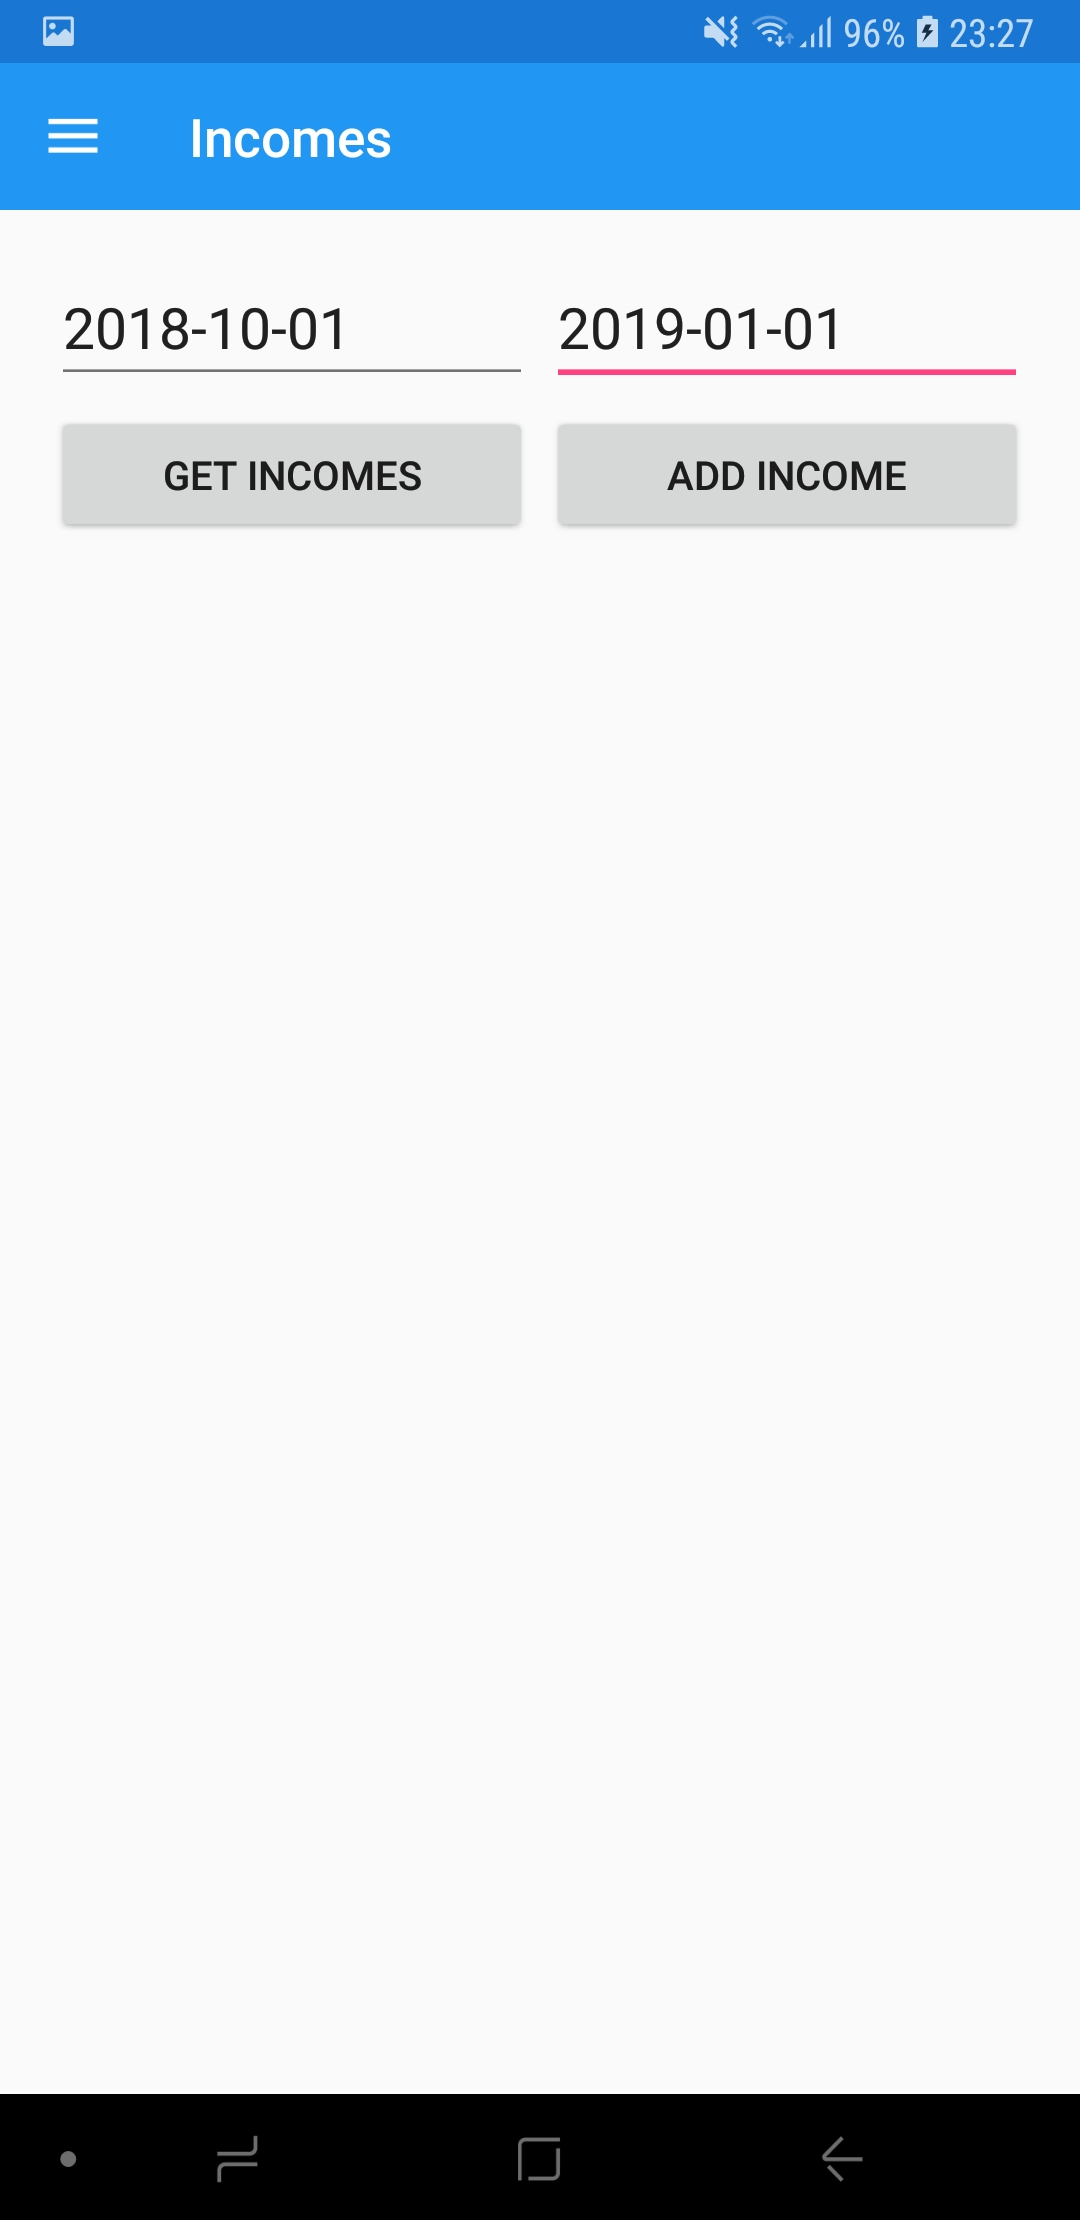
\includegraphics[width=1.75in]{img/mobile/przychody.jpg}
			\subcaption{Strona przychodów.\newline}
			\label{przychody_dodaj}
		\end{subfigure}
		\begin{subfigure}[b]{0.3\textwidth}
			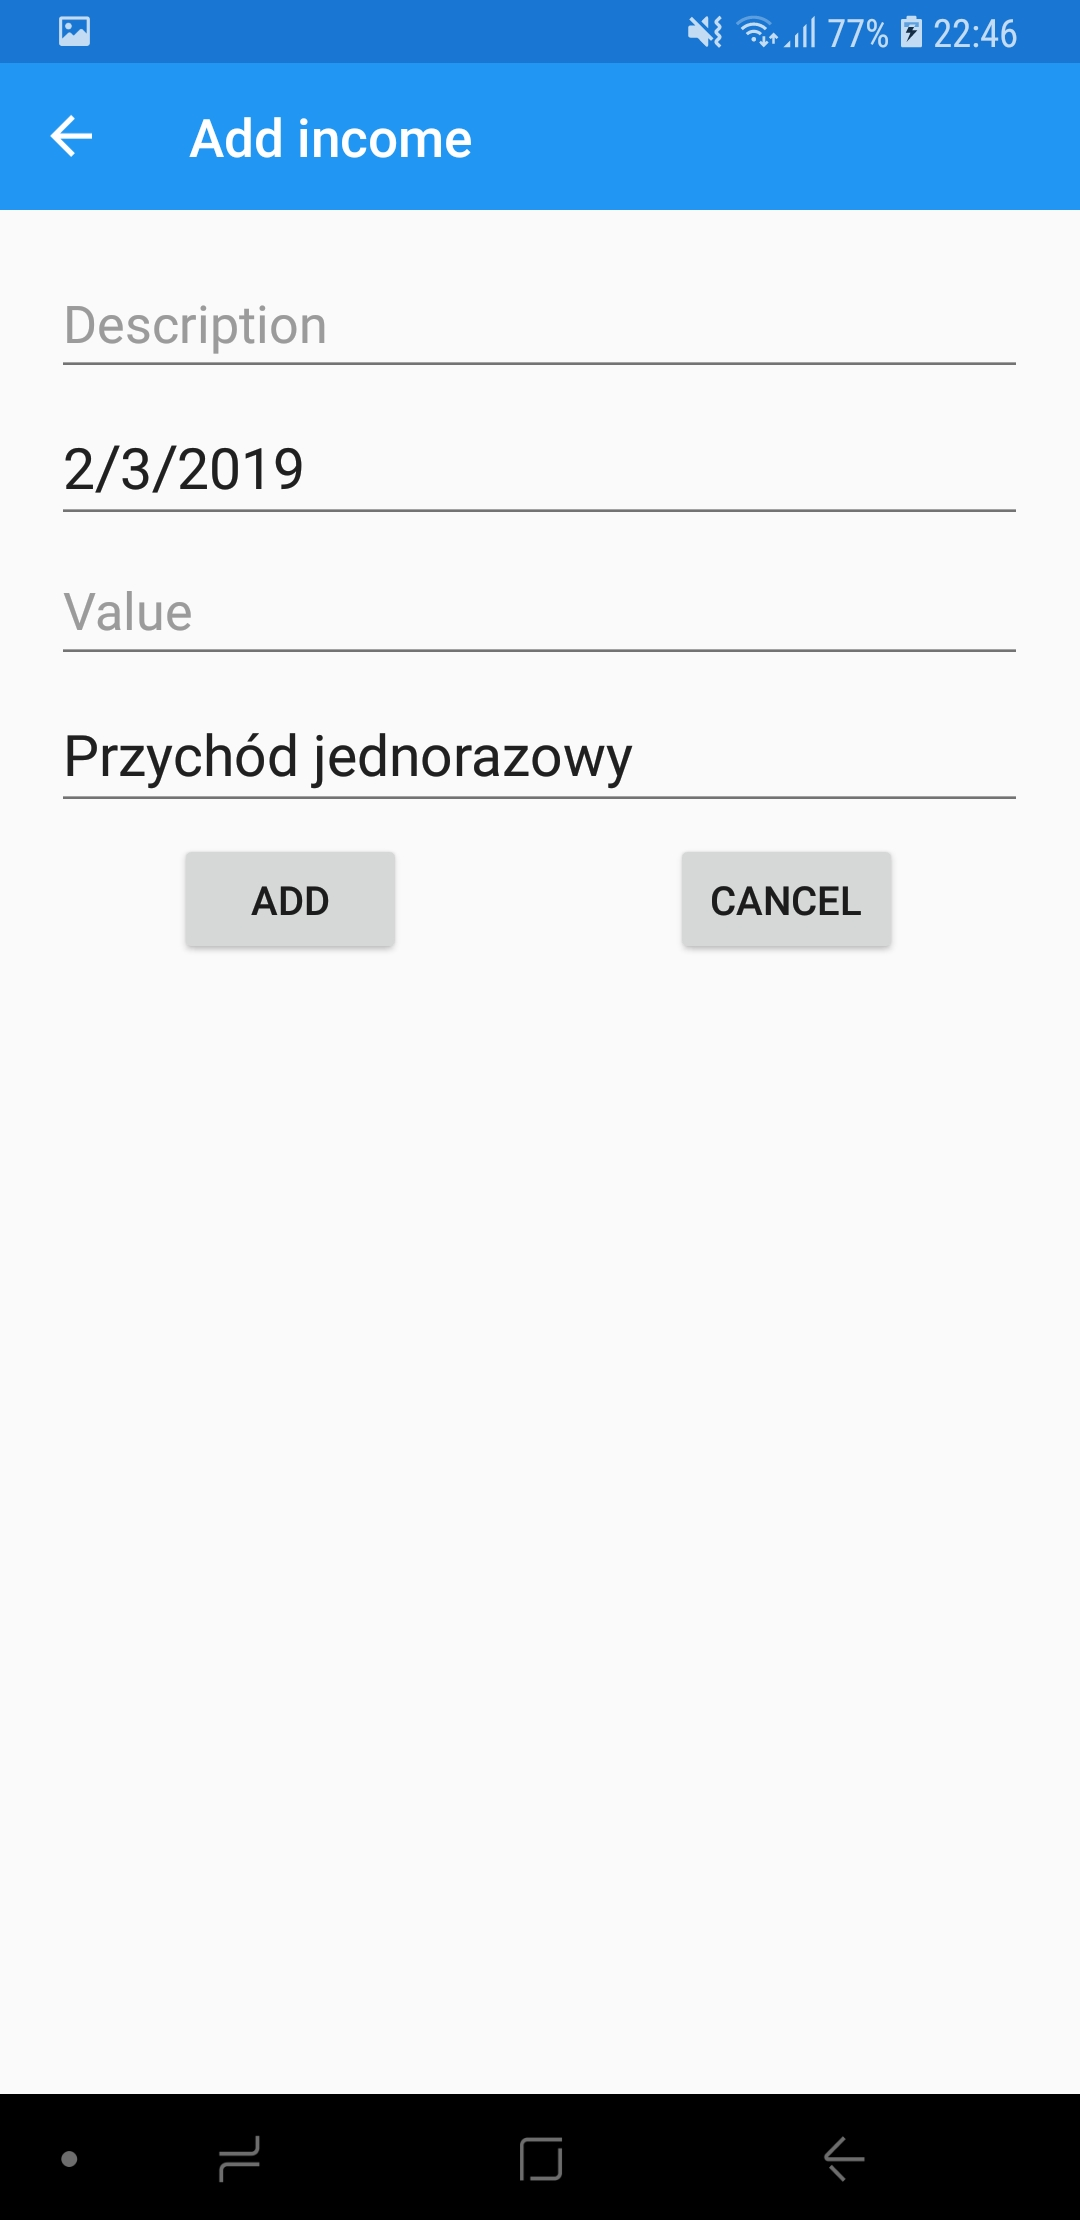
\includegraphics[width=1.75in]{img/mobile/dodaj_przychod.jpg}
			\subcaption{Formularz dodawania przychodu.}
			\label{dodaj_przychod}
		\end{subfigure}
	\end{center}
	\caption{Zrzuty ekranu procesu dodawania przychodu.}
\end{figure}

\textbf{Edycja przychodu} (przypadek użycia "edytuj przychód") - zmiana wartości, opisu lub kategorii istniejącego przychodu uwierzytelnionego użytkownika. W widoku listy przychodów (Rys. \ref{przychody_lista}), naciśnięcie konkretnego przychodu powoduje wyświetlenie menu z opcjami (Rys. \ref{przychod_menu}). Po naciśnięciu "Edit" wyświetla się formularz z edycją przychodu (Rys. \ref{przychod_edycja}), który, po wypełnieniu, można wysłać przyciskiem "SUBMIT", co powoduje zapisanie zmian, lub powrócić do listy przychodów przyciskiem "BACK".
\begin{figure}[!ht]
	\begin{center}
		\begin{subfigure}[b]{0.3\textwidth}
			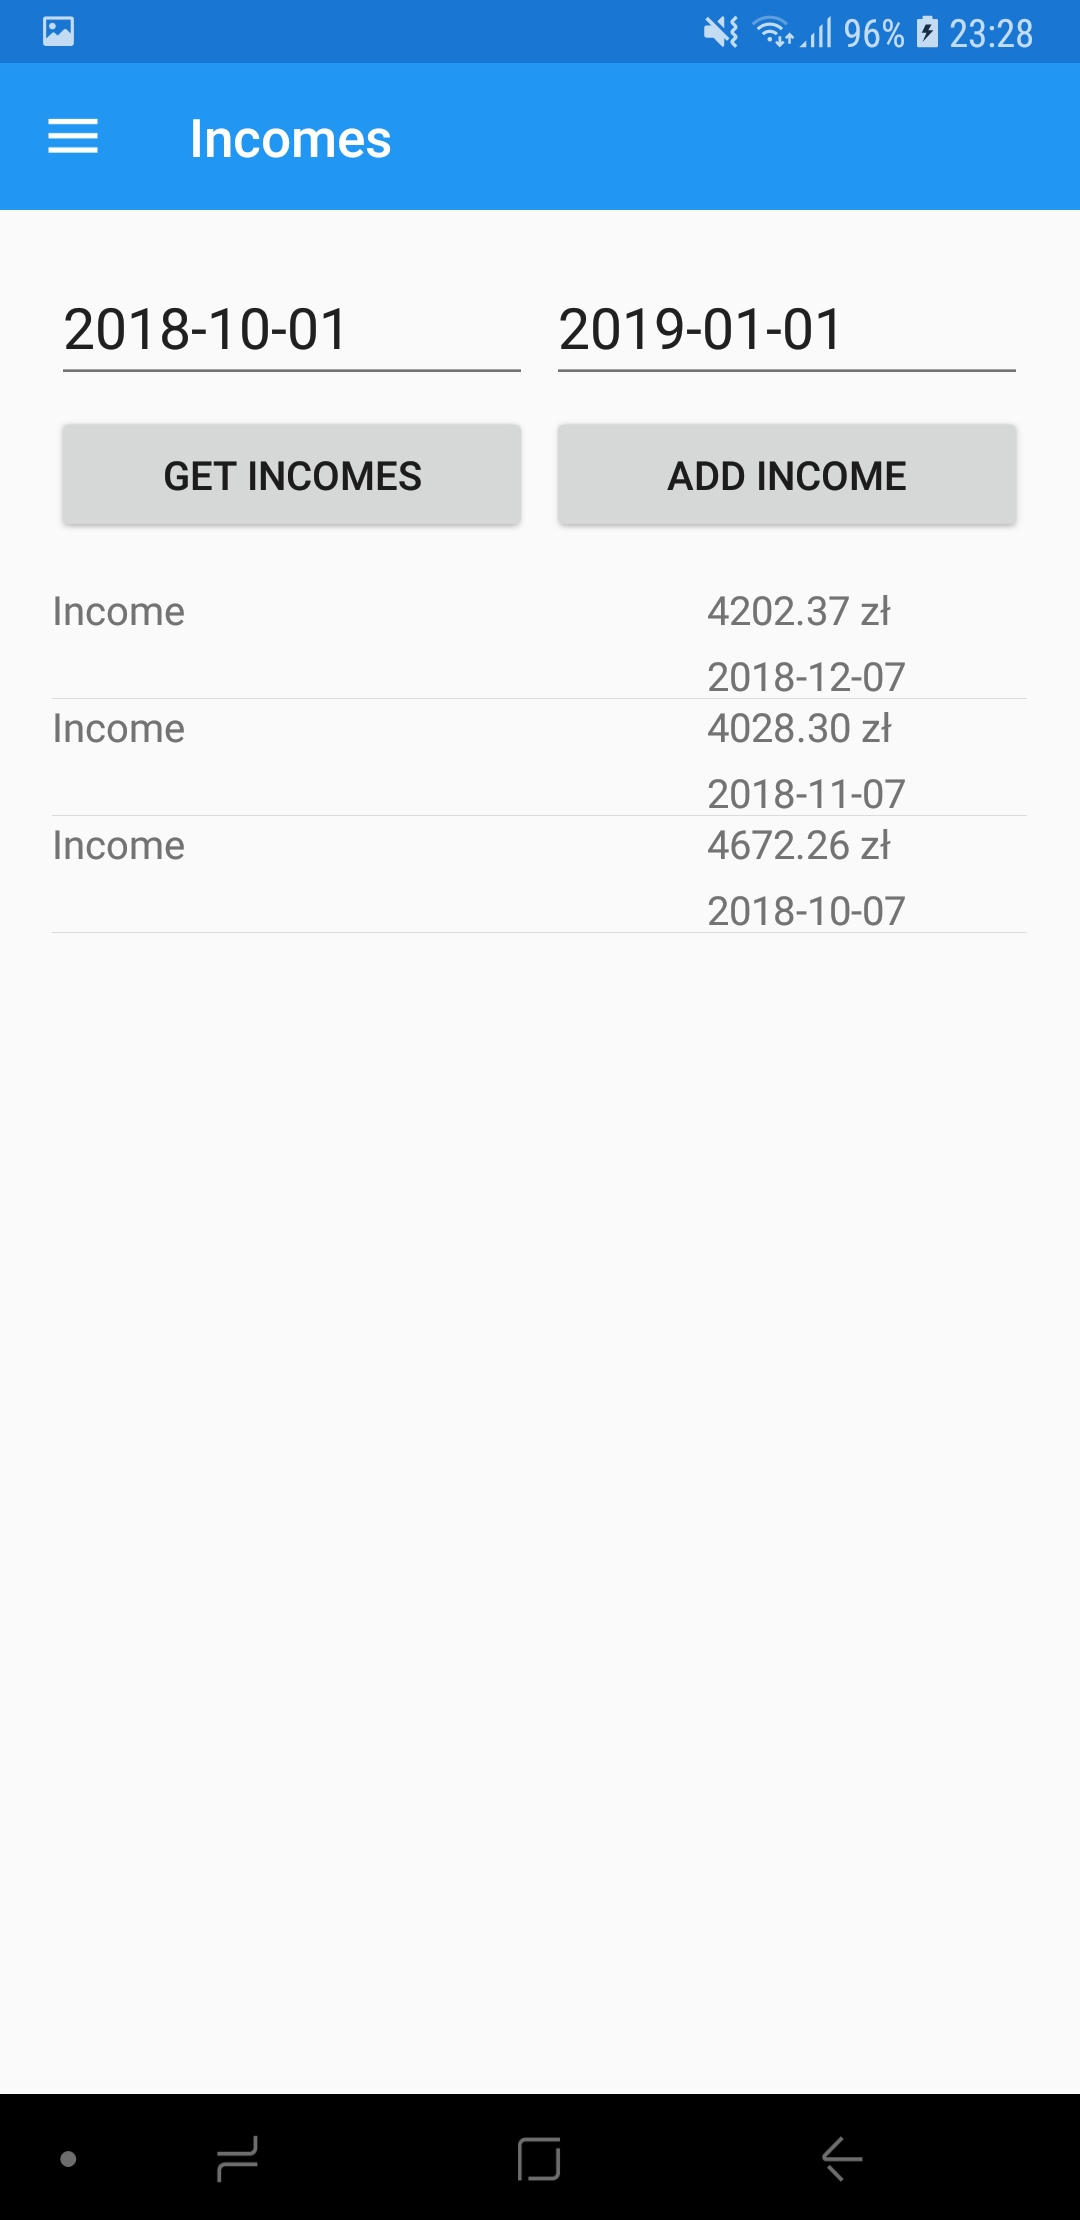
\includegraphics[width=1.75in]{img/mobile/przychody_gotowe.jpg}
			\subcaption{Lista przychodów.\newline}
			\label{przychody_lista}
		\end{subfigure}
		\begin{subfigure}[b]{0.3\textwidth}
			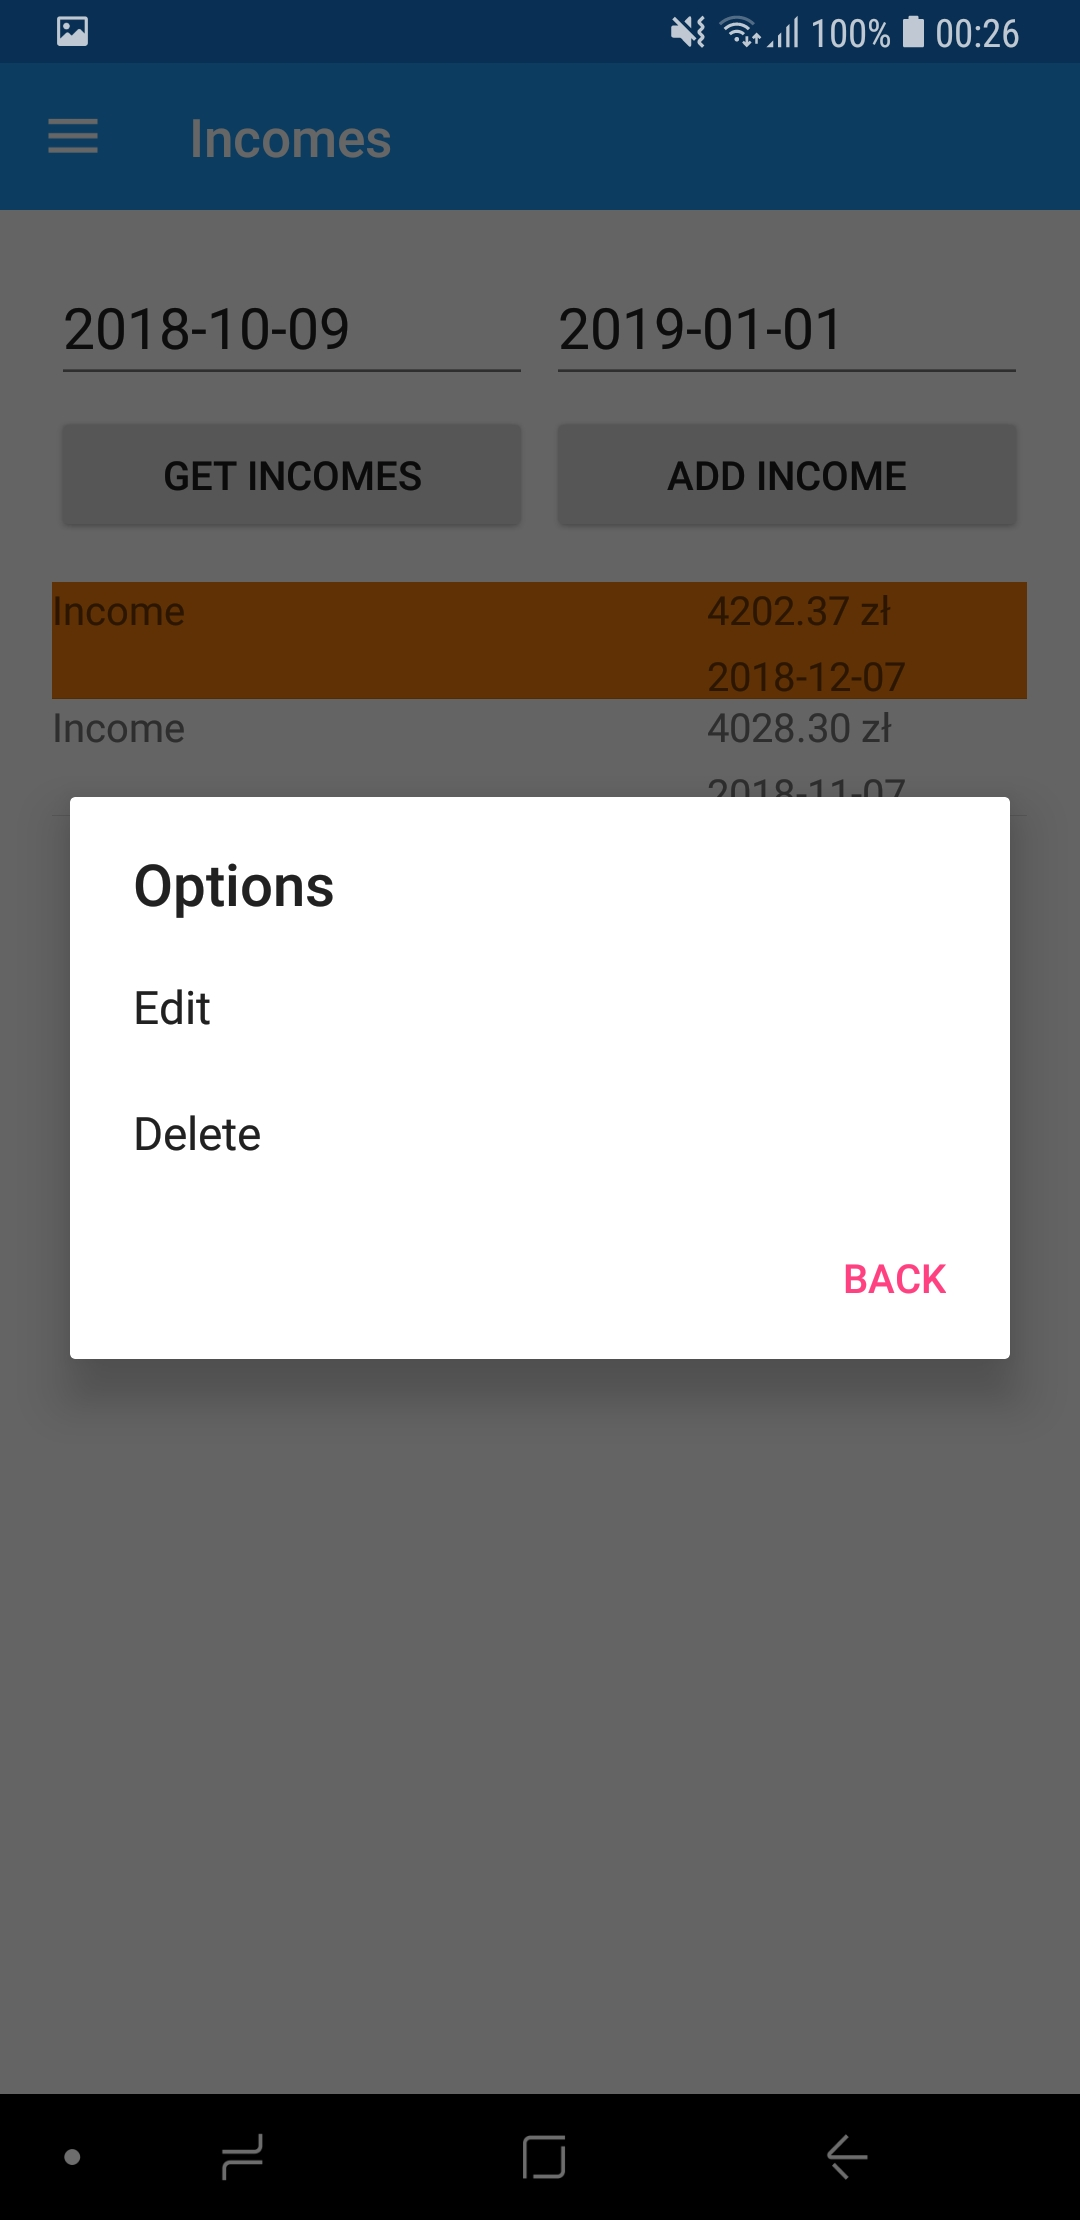
\includegraphics[width=1.75in]{img/mobile/przychod_menu.jpg}
			\subcaption{Menu przychodu.\newline}
			\label{przychod_menu}
		\end{subfigure}
		\begin{subfigure}[b]{0.3\textwidth}
			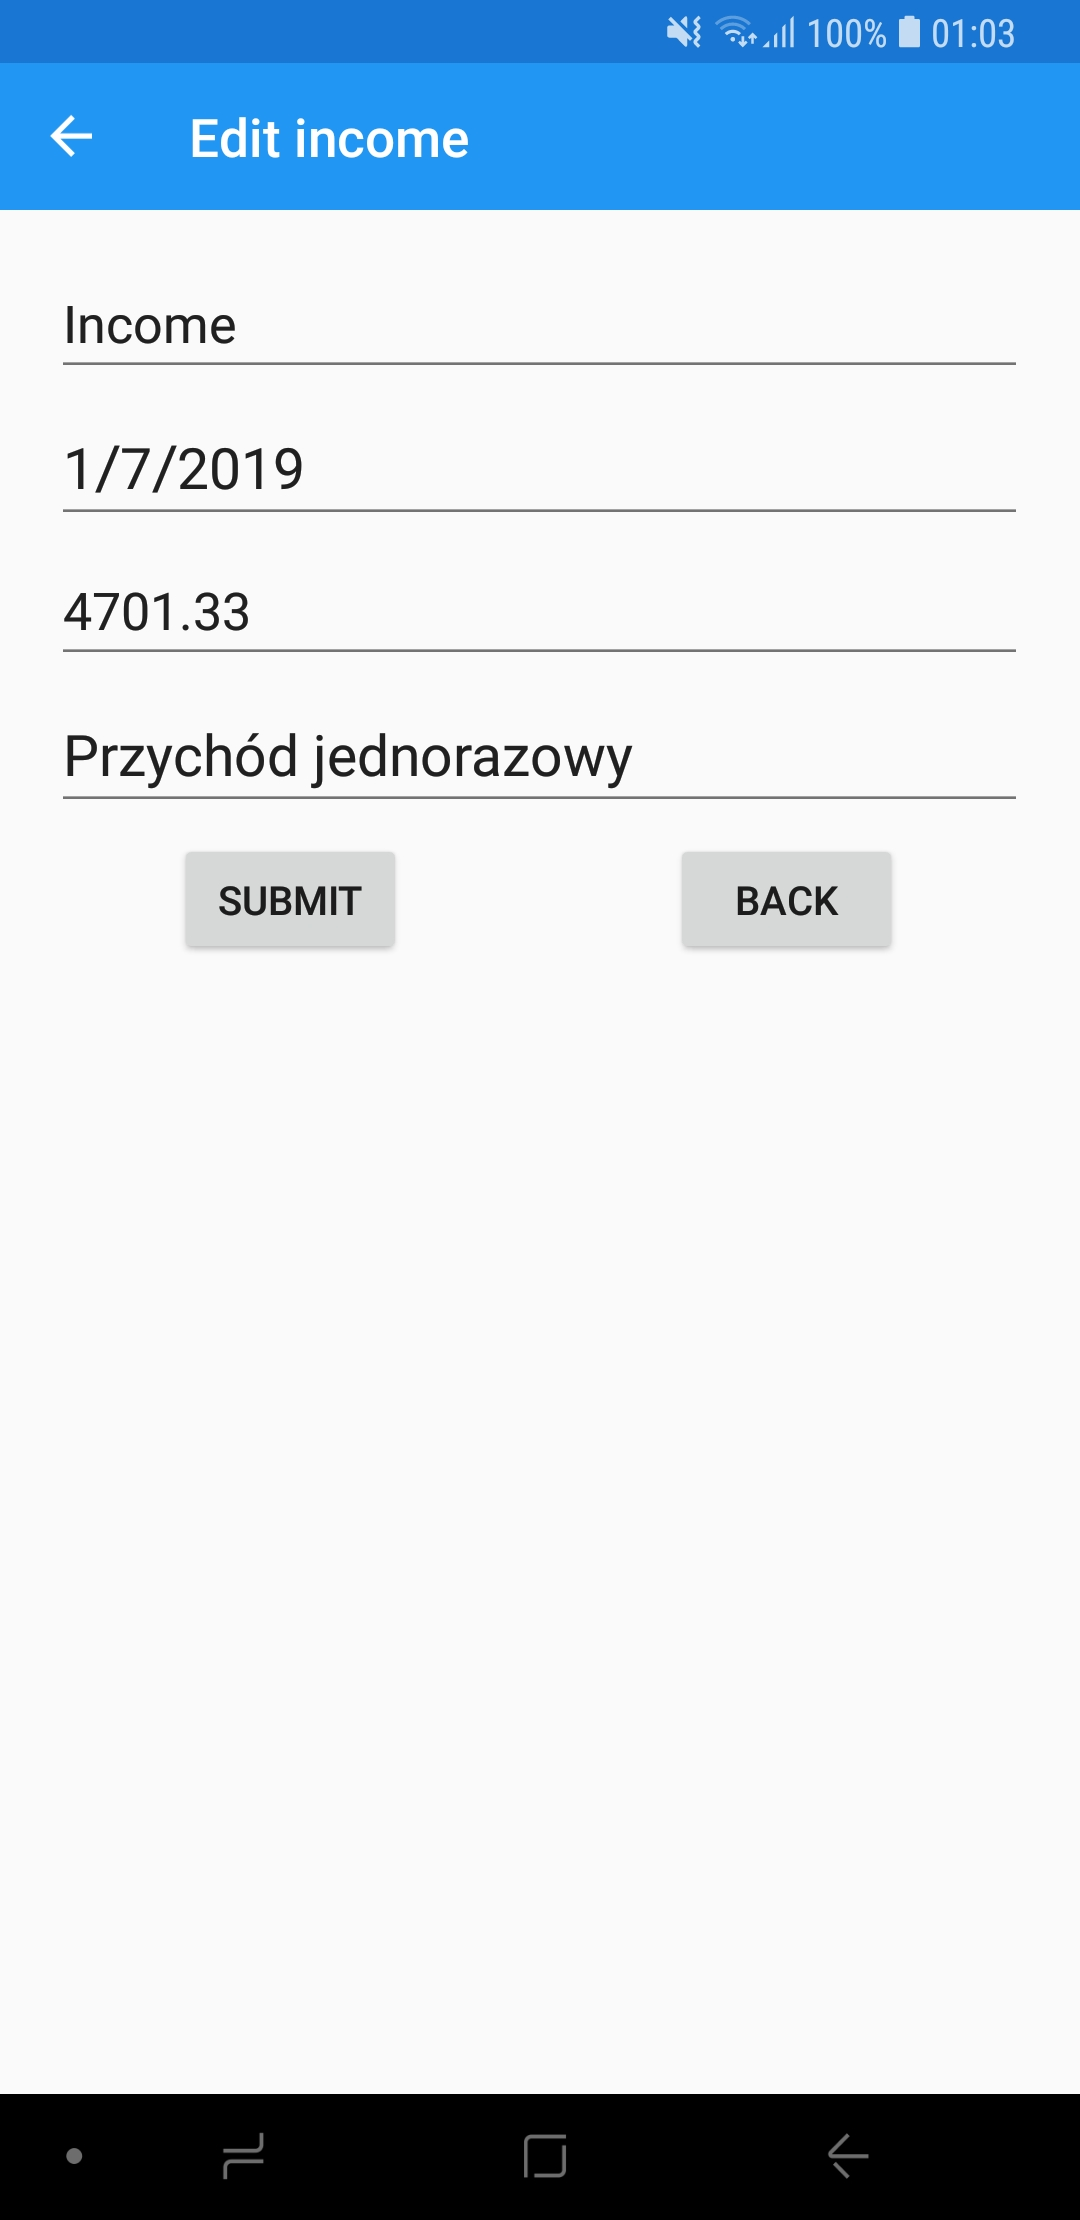
\includegraphics[width=1.75in]{img/mobile/przychod_edycja.jpg}
			\subcaption{Formularz edycji przychodu.}
			\label{przychod_edycja}
		\end{subfigure}
	\end{center}
	\caption{Zrzuty ekranu procesu edycji przychodu.}
\end{figure}

\textbf{Usuwanie przychodu} (przypadek użycia "usuń przychód") - usunięcie istniejącego przychodu należącego do aktualnie uwierzytelnionego użytkownika. Po naciśnięciu przychodu na liście przychodów (Rys. \ref{przychody_lista_usun}), wyświetlane jest menu (Rys. \ref{przychod_menu_usun}). Aby usunąć przychód należy w menu wybrać opcję "Delete" oraz potwierdzić chęć wykonania operacji (Rys. \ref{usun_na_pewno}).
\begin{figure}[!ht]
	\begin{center}
		\begin{subfigure}[b]{0.3\textwidth}
			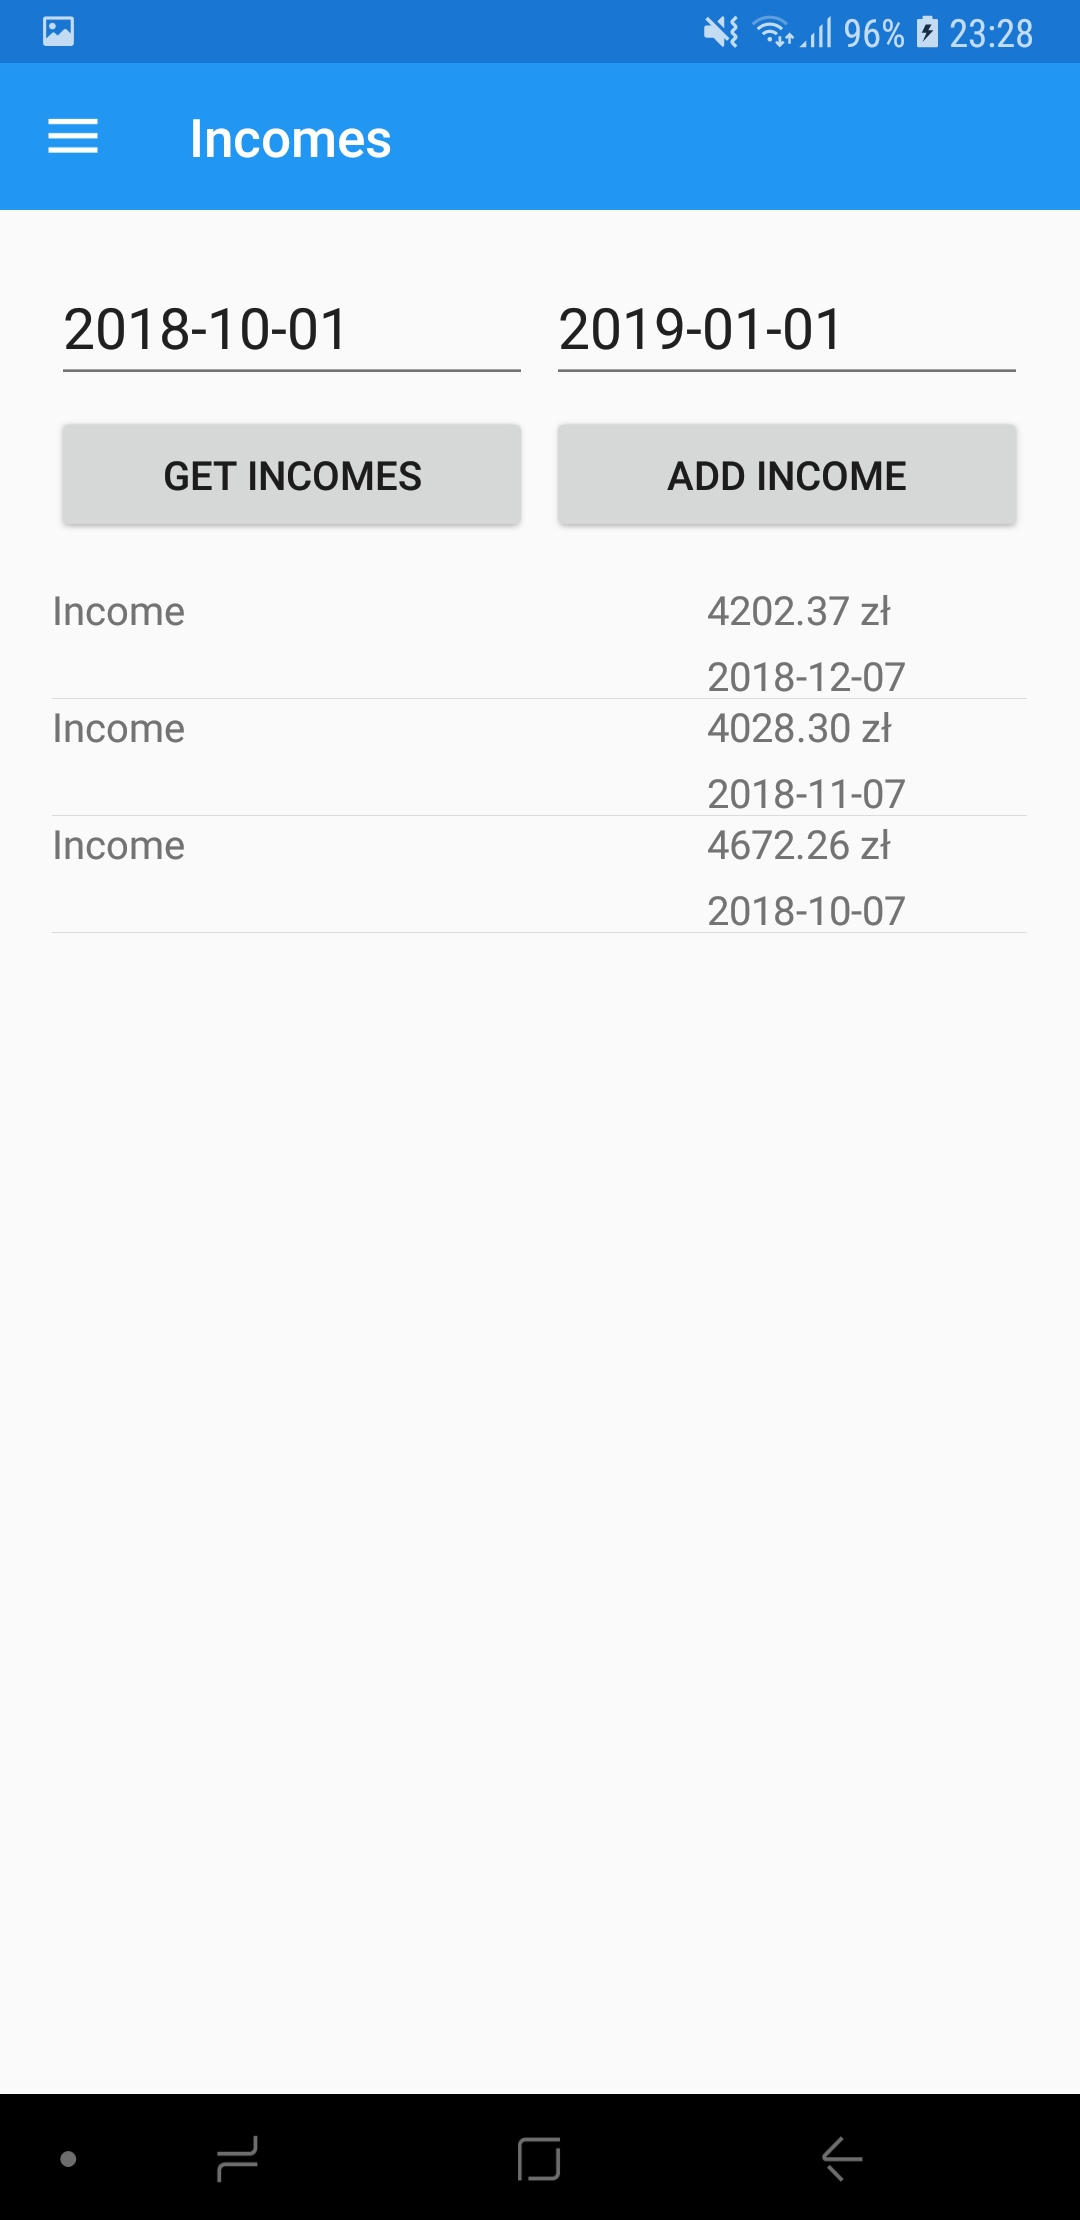
\includegraphics[width=1.75in]{img/mobile/przychody_gotowe.jpg}
			\subcaption{Lista przychodów.\newline}
			\label{przychody_lista_usun}
		\end{subfigure}
		\begin{subfigure}[b]{0.3\textwidth}
			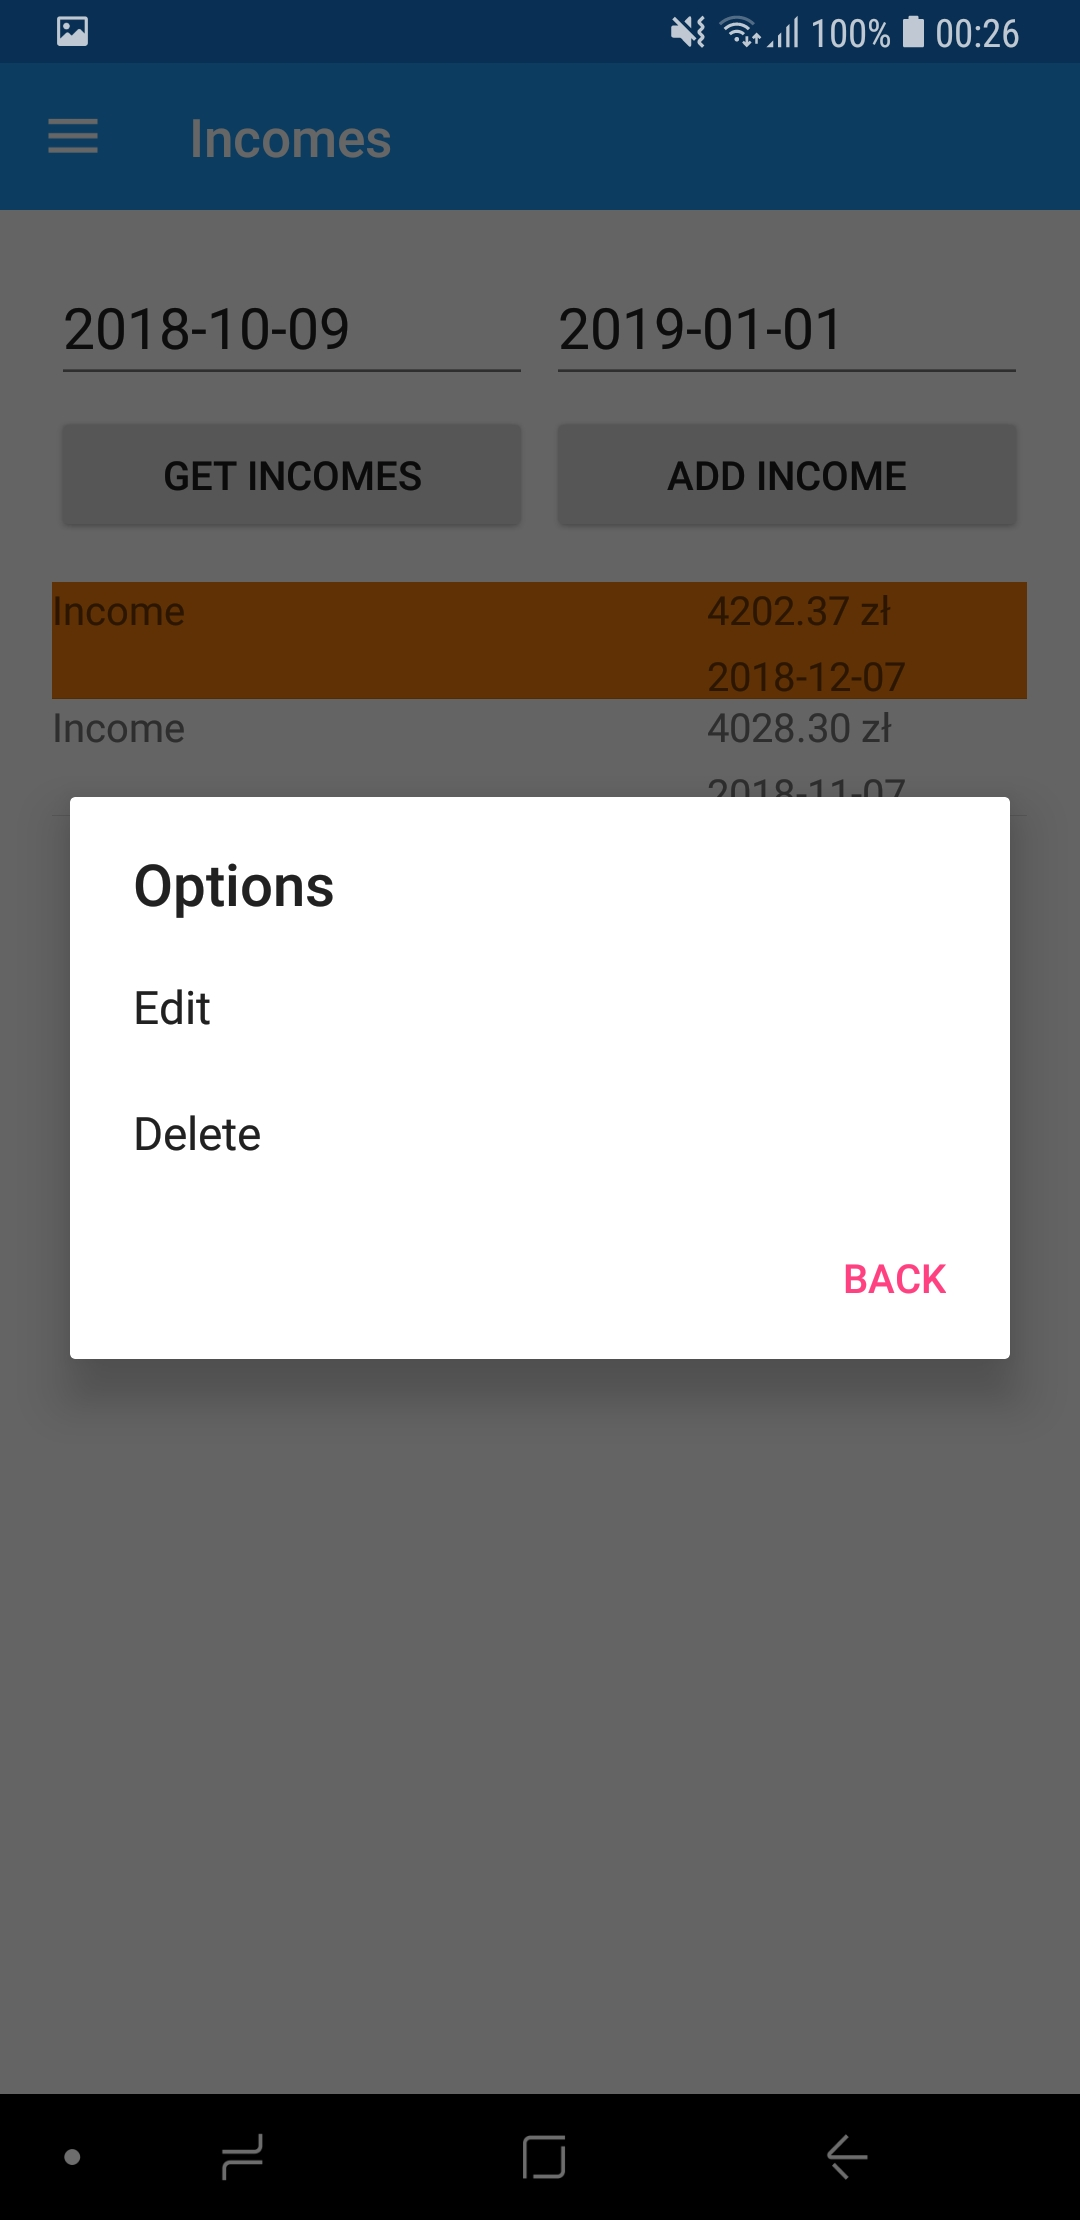
\includegraphics[width=1.75in]{img/mobile/przychod_menu.jpg}
			\subcaption{Menu przychodu.\newline}
			\label{przychod_menu_usun}
		\end{subfigure}
		\begin{subfigure}[b]{0.3\textwidth}
			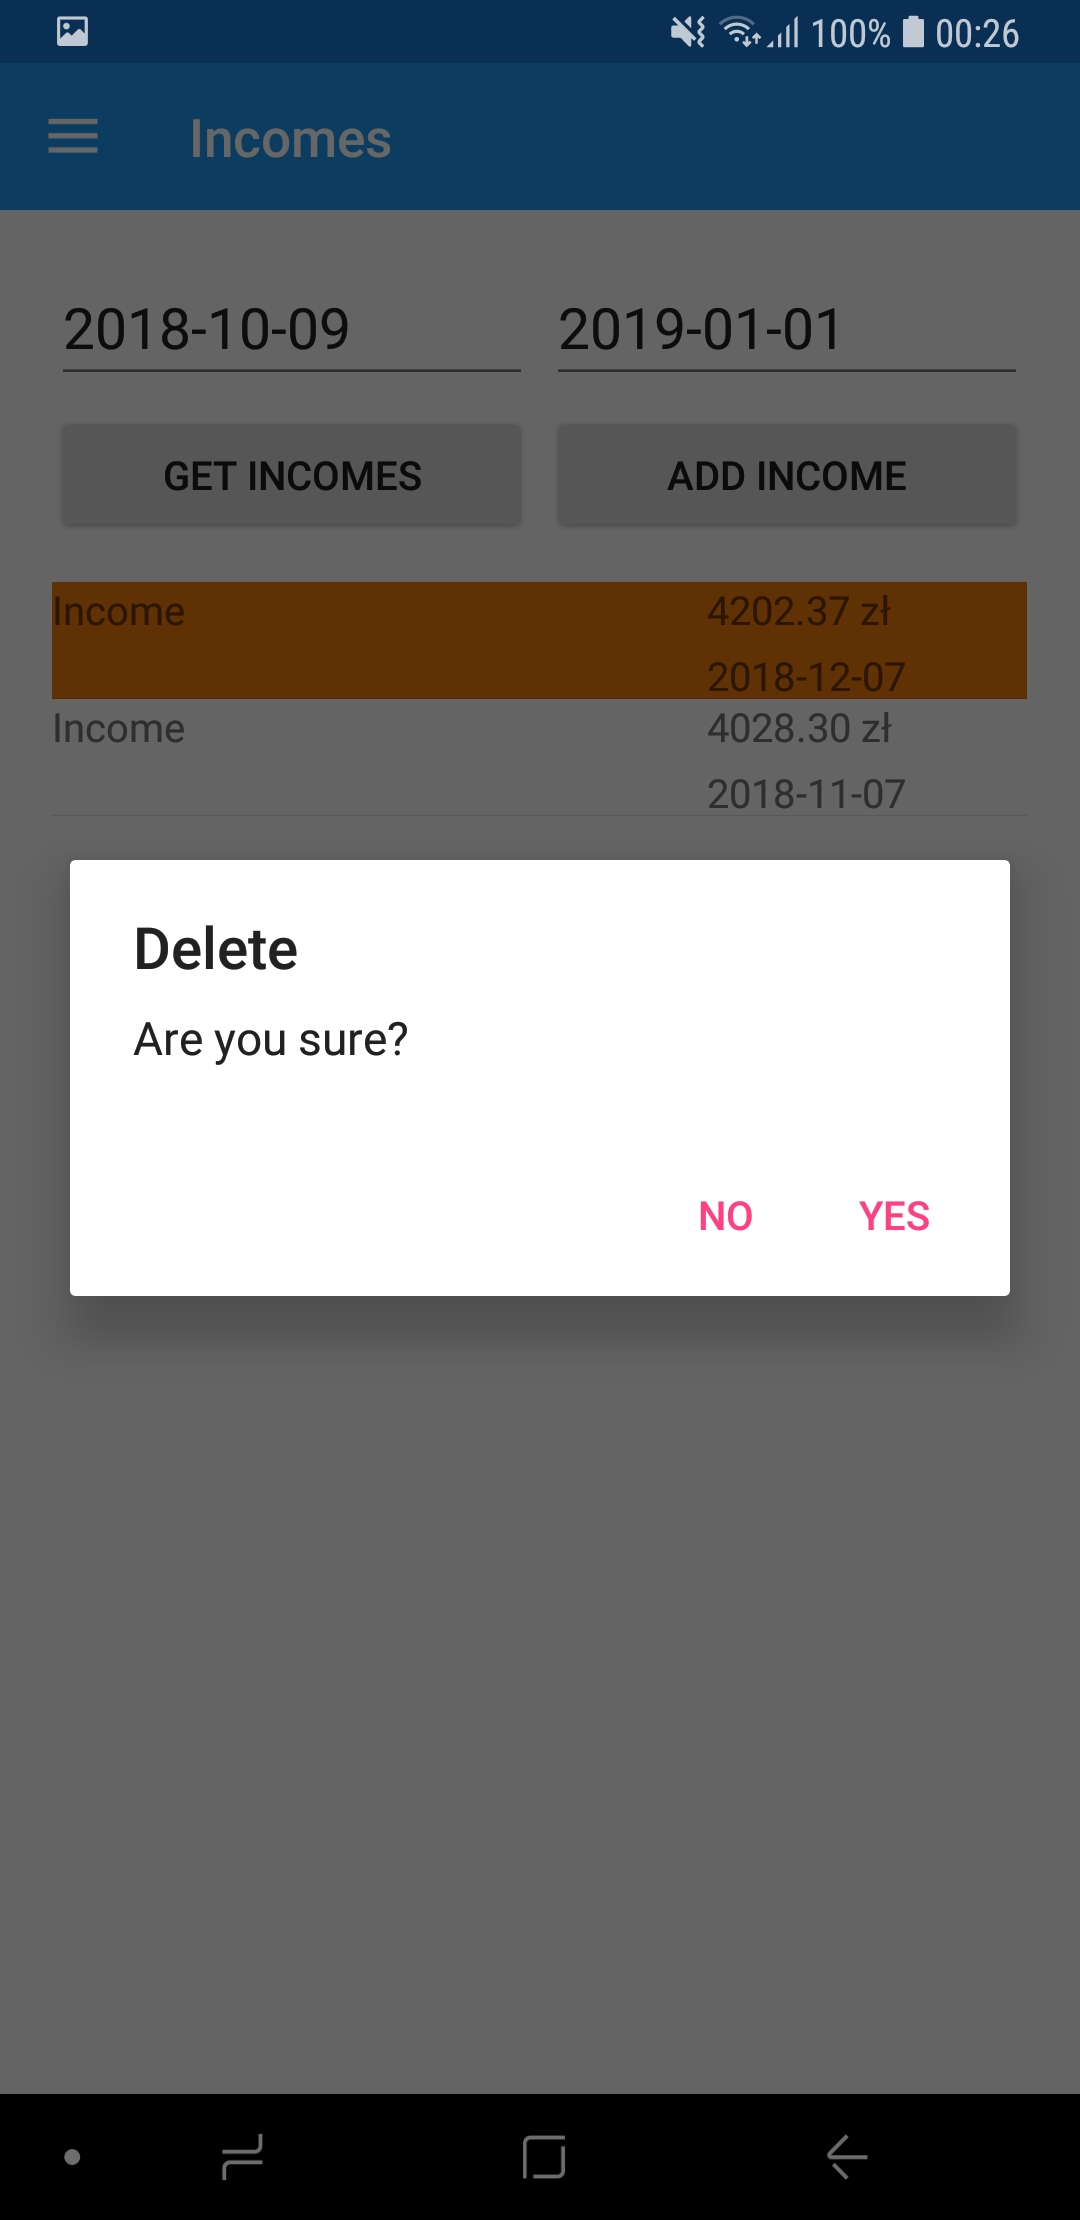
\includegraphics[width=1.75in]{img/mobile/usun_na_pewno.jpg}
			\subcaption{Okno potwierdzające chęć usunięcia przychodu.}
			\label{usun_na_pewno}
		\end{subfigure}
	\end{center}
	\caption{Zrzuty ekranu procesu usuwania przychodu.}
\end{figure}


\section{Moduł rejestracji wydatków}
W zakres modułu rejestracji wydatków wchodzą następujące przypadki użycia:
\begin{itemize}
	\item wyświetl swoje wydatki,
	\item dodaj wydatek,
	\item edytuj wydatek,
	\item usuń wydatek,
	\item wykonaj predykcję wydatków.
\end{itemize}

Operacje wyświetlania, dodawania, edycji oraz usuwania wydatków wykonuje się analogicznie do ich odpowiedników z modułu rejestracji przychodów.

\textbf{Predykcja wydatków} (przypadek użycia "wykonaj predykcję wydatków") jest to wykonanie prognozy wydatków powiązanych z wydatkiem głównym na nadchodzące miesiące. Po wybraniu z menu bocznego (Rys. \ref{hamburger_predykcja}) strony "Prediction" (Rys. \ref{predykcja}), uzupełnieniu wartości, daty oraz kategorii wydatku i naciśnięcie przycisku "PREDICTION" użytkownik otrzymuje prognozę wydatków na trzy nadchodzące miesiące (Rys. \ref{predykcja_gotowe}).
\begin{figure}[!ht]
	\begin{center}
		\begin{subfigure}[b]{0.3\textwidth}
			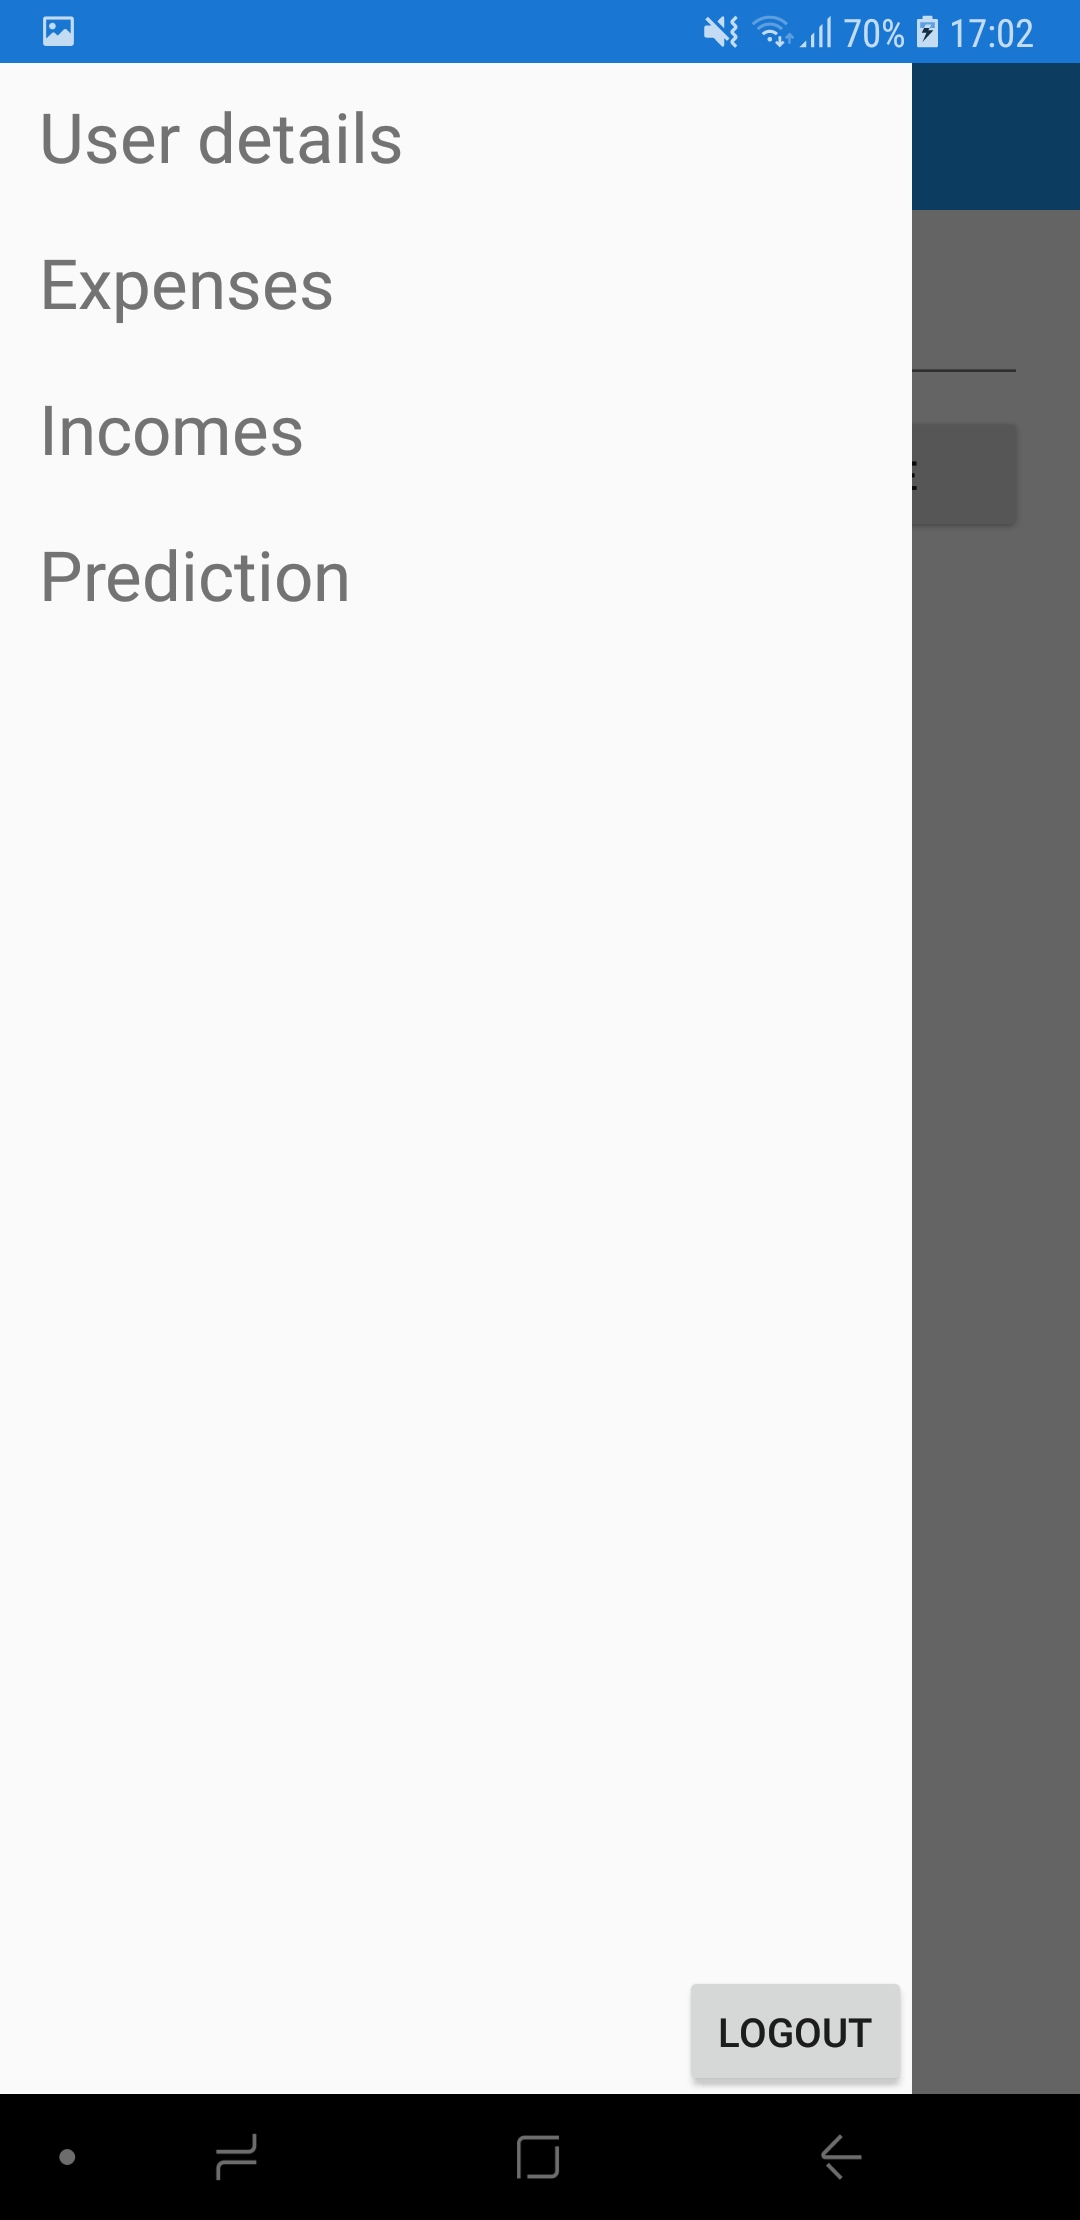
\includegraphics[width=1.75in]{img/mobile/menu_boczne.jpg}
			\subcaption{Menu boczne.}
			\label{hamburger_predykcja}
		\end{subfigure}
		\begin{subfigure}[b]{0.3\textwidth}
			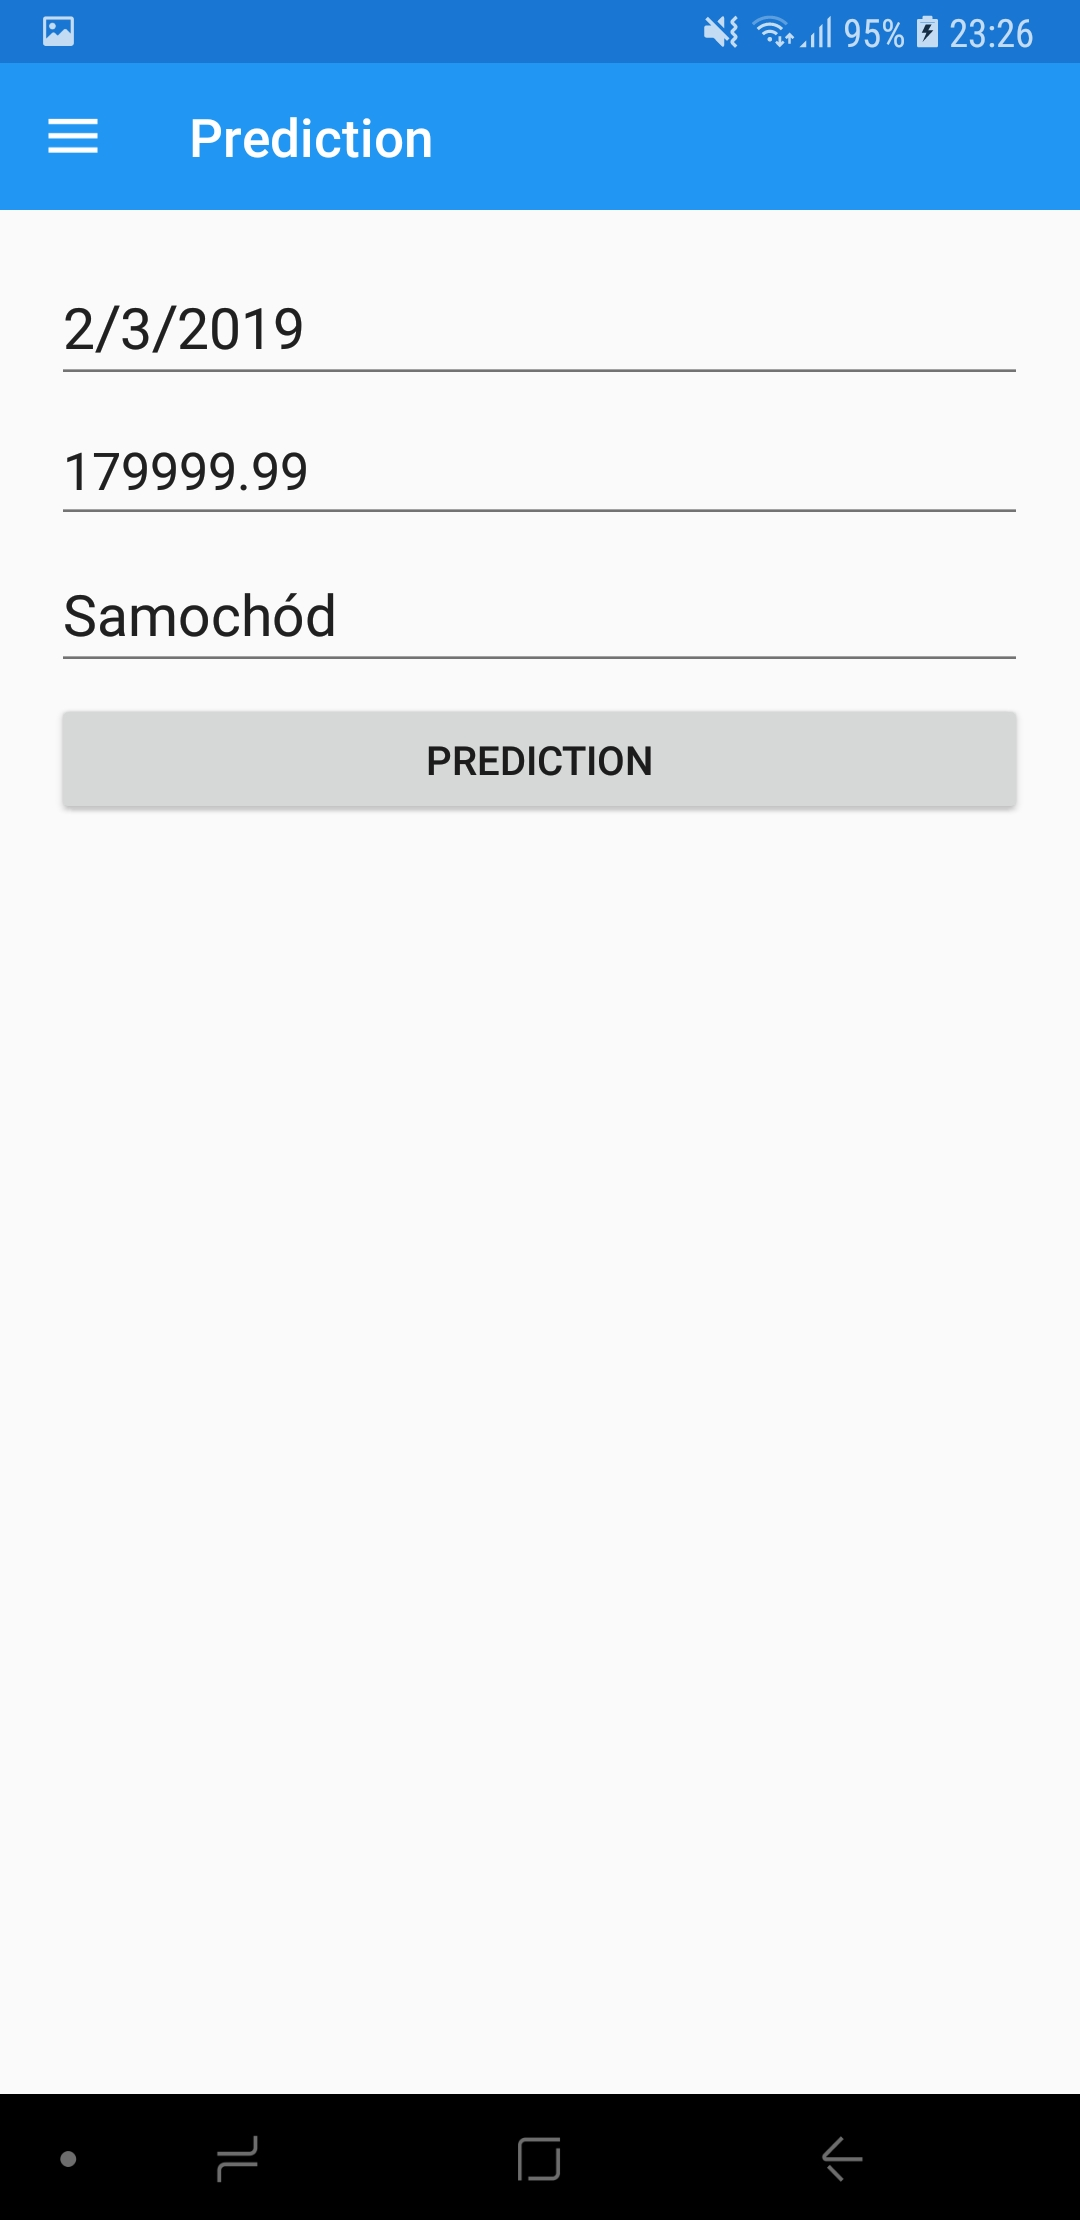
\includegraphics[width=1.75in]{img/mobile/predykcja.jpg}
			\subcaption{Strona predykcji.}
			\label{predykcja}
		\end{subfigure}
		\begin{subfigure}[b]{0.3\textwidth}
			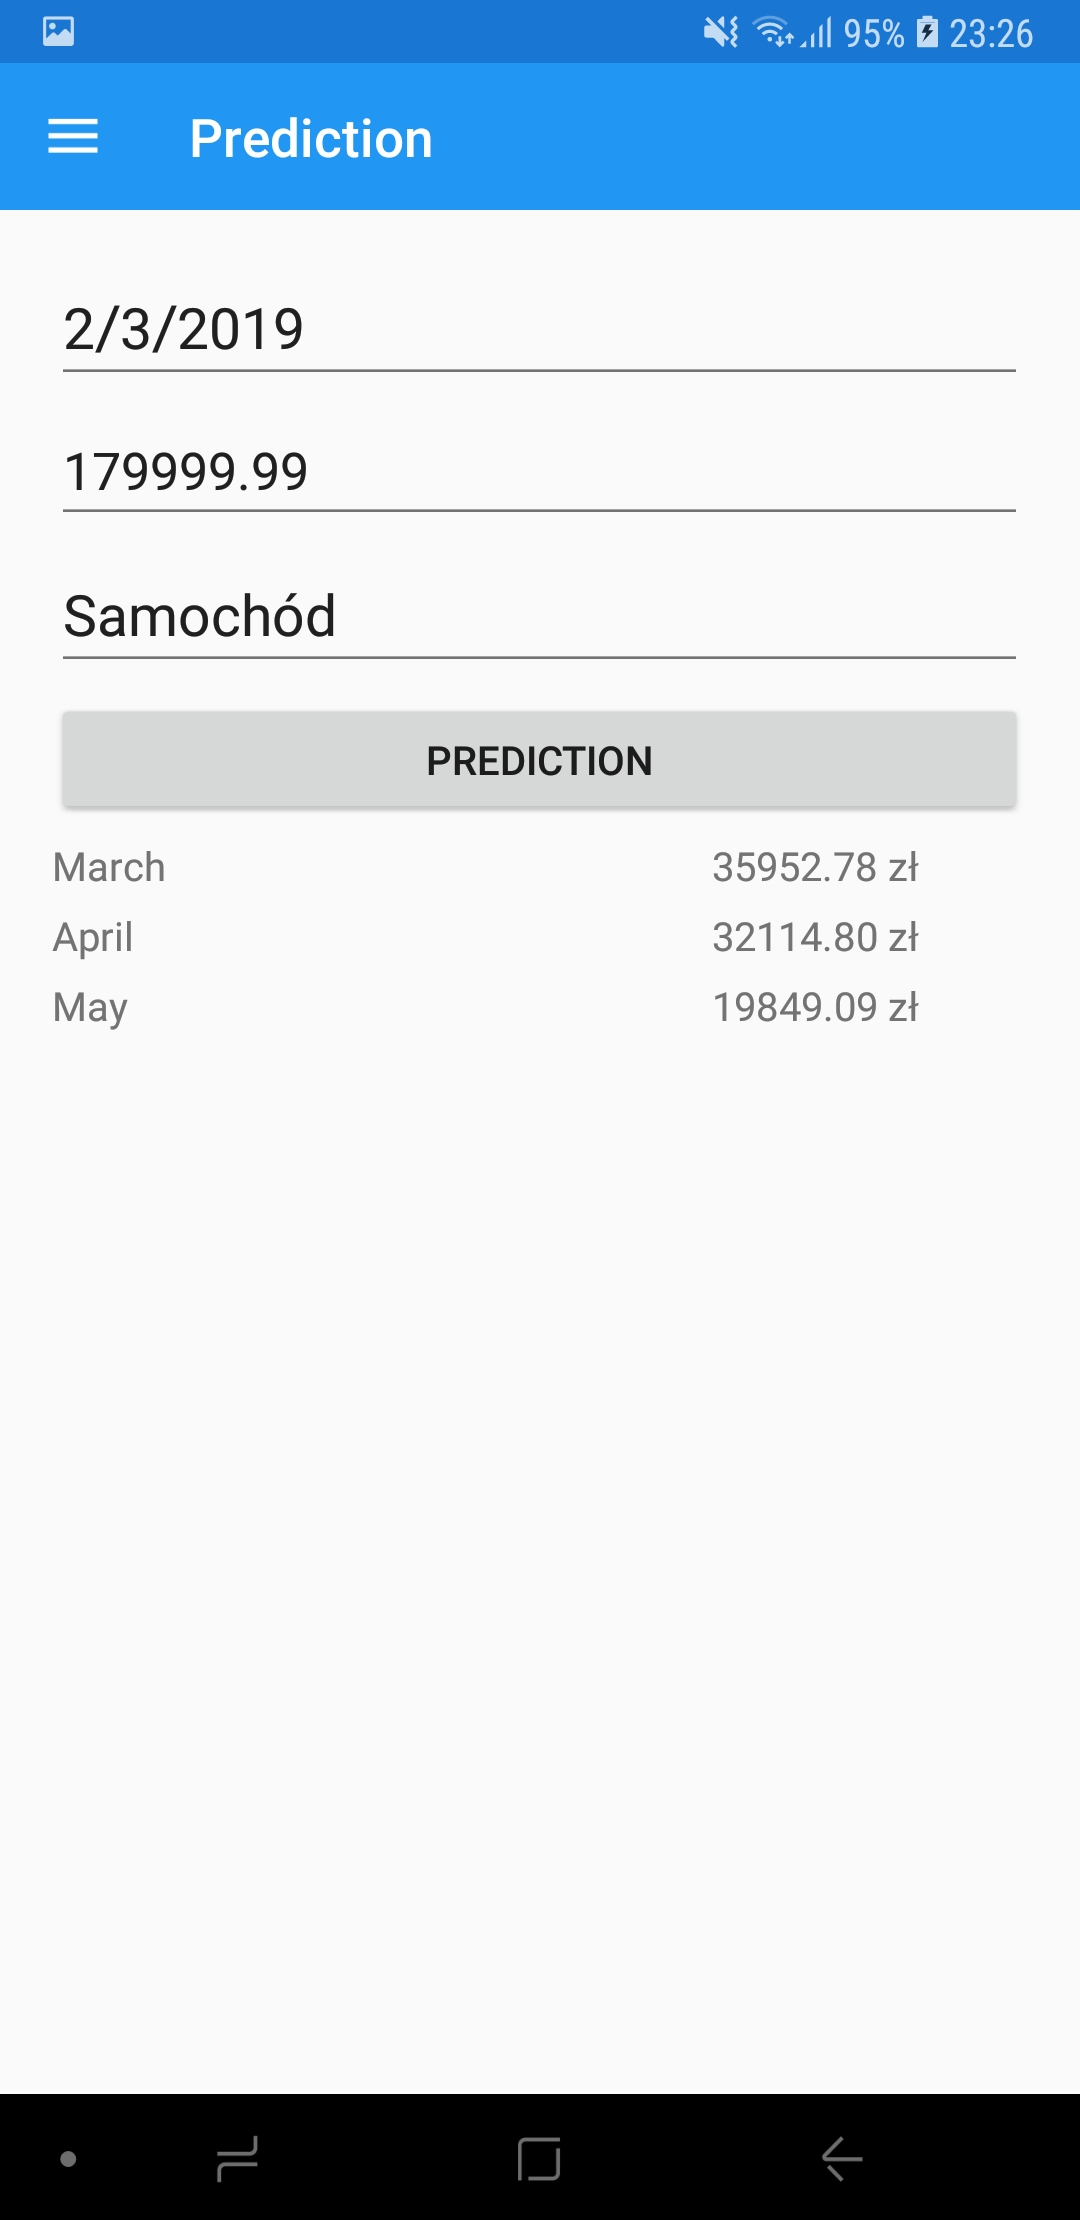
\includegraphics[width=1.75in]{img/mobile/predykcja_gotowe.jpg}
			\subcaption{Wyniki predykcji.}
			\label{predykcja_gotowe}
		\end{subfigure}
	\end{center}
	\caption{Zrzuty ekranu procesu wykonywania predykcji wydatków.}
\end{figure}